% Formato modificado por CORUM para la escritura de artículo

% Si es formato ieee descomentar la siguiente linea
\documentclass[journal,transmag]{IEEEtran}

\usepackage[utf8]{inputenc}
%\usepackage[spanish]{babel}
\usepackage{amsmath}
\usepackage{amsfonts}
\usepackage{amssymb}
\usepackage{graphicx}
%\usepackage[colorlinks,hyperindex,linkcolor=red,urlcolor=blue]{hyperref}
\usepackage{hyperref}
\usepackage{setspace}
\usepackage{subfig}
\usepackage{url}         

\usepackage{epsfig}

%ruta para guardar las imagenes
\graphicspath{ {figuras/} }

\begin{document}
\title{Plataforma educativa de sexualidad para el proyecto ``Red Sentir... Con-ciencia juvenil''}

% author names and affiliations IEEE
% use a multiple column layout for up to three different
% affiliations

%\author{\IEEEauthorblockN{J. A. Gómez Múnera$^{\ast }$ y A. Giraldo$^{\ast }$}
%\IEEEauthorblockA{$^{\ast }$Corporación Estudiantes Universitarios y Profesionales de Marinilla (CORUM)
%\\Calle 30 San José N$\circ$ 25-118, Marinilla - Antioquia, Colombia
%\\ \href{mailto:gomezmunera@corum.org.co}{gomezmunera@corum.org.co}, \href{mailto:alejo@corum.org.co}{alejo@corum.org.co}}
%}

\author{\IEEEauthorblockN{J. A. Gómez Múnera\IEEEauthorrefmark{1,2}, and
A. Giraldo\IEEEauthorrefmark{1,2}}
\IEEEauthorblockA{\IEEEauthorrefmark{1}Corporación Estudiantes Universitarios y Profesionales de Marinilla (CORUM) \\Calle 30 San José N$\circ$ 25-118, Marinilla - Antioquia, Colombia}
\IEEEauthorblockA{\IEEEauthorrefmark{2}Instituto Tecnológico COREDI \\ Calle 30 N$\circ$ 36-11, Marinilla - Antioquia, Colombia
\\ \href{mailto:gomezmunera@corum.org.co}{gomezmunera@corum.org.co}, \href{mailto:alejo@corum.org.co}{alejo@corum.org.co}}
\thanks{Manuscript received December 1, 2018; revised August 26, 2015. 
Corresponding author: J. A. Gómez(email: gomezmunera@corum.org.co)}}

% The paper headers
\markboth{Transactions on Education ,~Vol.~14, No.~8, December~2018}%
{Gómez \MakeLowercase{\textit{et al.}}: Bare Demo of IEEEtran.cls for IEEE Transactions on Magnetics Journals}

% make the title area
\maketitle

\begin{abstract}
\textbf{\textit{Abstract}}---Dentro del plan nacional de desarrollo 2014-2018 de Colombia se planteó la educación como un pilar fundamental, donde el mismo plan sirviera como un mecanismo que permitiera una igualdad social y así nivelar las posibilidades de todos los Colombianos. Teniendo esto en cuenta, y al considerar el incremento acelerado en el uso de las tecnologías de la información y la comunicación, junto con la posibilidad de brindar una mayor cobertura en educación, como la corporación de estudiantes universitarios y profesionales de Marinilla (CORUM) desarrolló e implementó un proyecto llamado ``Red Sentir...Con-ciencia juvenil'' centrado en la prevención de embarazo adolescente, fortalecimiento del plan de vida, pensamiento crítico, autonomía y toma de decisiones conscientes. El proyecto se deriva en tres componentes fundamentales que constituyen un proceso de formación integral con jóvenes entre 10 y 19 años del oriente Antioqueño, que les permite interactuar y relacionarse con padres, maestros y agentes institucionales. Los componentes mencionados son: $(i)$ formación y socialización, $(ii)$ mesa regional, y $(iii)$ una plataforma digital. En el presente artículo se hace énfasis en las estrategias y desarrollos realizados por el componente digital en la creación de un entorno virtual que permite vincular expertos, maestros, jóvenes, padres de familia e instituciones de salud. Para el desarrollo se creó una red social a través de diferentes tecnologías, que involucran desarrollo web, creación de bases de datos relacionales, configuración de servidores y desarrollo de videojuegos. Todas esto posible a través de distintos lenguajes de programación tales como, python, HTML, javascript, que configuran aplicaciones tanto desde el lado del cliente como aplicaciones desde el lado del servidor.
\end{abstract}

\begin{IEEEkeywords}
Plataforma educativa, educación sexual, embarazo en adolescencia, servicios de planificación familiar, servicios de salud para adolescentes, servicios de salud sexual y reproductiva, educación sexual.
\end{IEEEkeywords}

%\IEEEdisplaynontitleabstractindextext
\IEEEpeerreviewmaketitle

\section{INTRODUCCIÓN}

En Colombia la fecundidad en la adolescencia se convirtió en un problema de salud pública, cuando a partir de 1990 (para adolescentes entre 15 y 19 años) se encontraron medidas de un $12.8\%$, presentando  en los años posteriores una tendencia sistemáticamente creciente que encuentra el valor máximo en 2005 ($20.5\%$). Para el año 2010 ($19.5\%$) se logró una tendencia decreciente que se continua presentando en el 2015 con una medida del $17.4\%$. Se espera que para el año 2021 según el ajuste realizado al Plan Decenal de Salud Pública 2012-2021 se llegue a la disminución de ese porcentaje a un $15\%$~\cite{Pro2015}. Por tal motivo, Colombia se planteó en los objetivos de desarrollo del milenio (ODM) tener tazas de embarazo adolescente por debajo del $15\%$, sin embargo los porcentajes alcanzados fueron muy alejados de esas cifras, lo cual hace necesario redoblar los esfuerzos que permitan disminuir embarazo en adolescentes. En 2013 Colombia registró 6.423 nacimientos en mujeres entre los 10 y 14 años y casi 150 mil en mujeres entre los 15 y 19 años, cifra que es elevada si se tiene en cuenta que en conjunto representan el $23.5\%$ del total de nacimientos~\cite{PNUD2015}.

Los esfuerzos por reducir el embarazo adolescente han sido más significativos en los grupos más favorecidos socialmente, en contraposición con los menos favorecidos provocando que se amplíen las brechas socioeconómicas. Esto refleja la  necesidad de realizar mayores esfuerzos de la política de prevención del embarazo adolescente en los grupos menos favorecidos socialmente y donde se ha identificado la mayor prevalencia del embarazo adolescente~\cite{Pro2015, Pro2015II}: zonas rurales, menos educados, situaciones de pobreza. 

Las diferencias ocasionadas por las situaciones socioeconómicas y por la ubicación geográfica, ponen en evidencia que se deben tomar acciones o generar estrategias de inclusión social~\cite{BID2017}, en el que se aborden las temáticas de educación sexual de manera transversal con un enfoque de derechos y con una mayor cobertura, para permitir así la reducción de las brechas existentes confirmadas en el plan nacional de desarrollo 2014-2018, y  el  principio  de  “no  dejar  a  nadie  atrás”  consagrado  en  la  Agenda  2030,  que  comprende a los Objetivos de Desarrollo Sostenible (ODS).

La problemática del embarazo adolescente en Colombia demuestra que solo el $9\%$ de las mujeres y el $5\%$ de los hombres jóvenes consultan los servicios de salud debido a la desconfianza y desconocimiento de este sistema. A pesar de que los adolescentes son conscientes de los métodos anticonceptivos, tan sólo una pequeña porción los usan, según cifras publicadas en~\cite{Pro2015II}, para el rango de edad entre 15-19 años, en las mujeres es alrededor del $30\%$ y en los hombres del $47\%$. El uso de métodos anticonceptivos no solo es importante para controlar los crecimientos de natalidad del país, sino también para prevenir infecciones de transmisión sexual, en este sentido, el uso del condón en Colombia es una de las prácticas más seguras para prevenir las enfermedades de transmisión sexual ($85.1\%$ en hombres y $84.4\%$ en mujeres).

Cuando se aborda la problemática desde un enfoque de derechos y para dar respuesta a las necesidades de información sobre la educación en temas de sexualidad y reproducción, es necesario plantear la educación de una manera integral, en el que se potencien y fomenten el empoderamiento y se desarrollen habilidades en los jóvenes desde una perspectiva crítica que les permita tomar decisiones que posibiliten el cumplimiento efectivo de sus derechos sexuales y reproductivos. La sexualidad es un derecho humano, cuya construcción efectiva requiere de procesos o estrategias intencionadas, estructuradas y sistemáticas que faciliten el acceso a información sobre temas referentes a la sexualidad analizada en los diferentes entornos geográficos y socioeconómicos más allá del vivido en la escuela.

En Colombia el derecho a la educación sexual hace parte integral tanto de la Constitución Política de 1991 como de las diversas políticas que desarrollan los acuerdos, pactos, conferencias, convenios y convenciones internacionales ratificados por el Estado. El rol del sector educativo en la promoción y garantía de los Derechos Sexuales y Derechos Reproductivos se destaca a partir de la Resolución 3353 de 1993. Por ende, el carácter obligatorio de la educación sexual en las instituciones educativas se ratifica en el Plan Nacional de Educación Sexual (MEN, 1994) y la Ley General de Educación (Ley  115  de 1994 y Decreto reglamentario 1860). Otros referentes normativos son el documento CONPES Social 147, donde se definen los lineamientos para la prevención del embarazo en la adolescencia, el PDSP 2012-2021 (MSPS, 2014), en el cual  se  establece que la sexualidad es una de las dimensiones priorizadas, es decir, considera este aspecto como fundamental para lograr la salud y el bienestar de todo individuo, sin distinción por sexo, género, etnia, ciclo de vida, nivel socioeconómico o cualquier otro aspecto diferencial~\cite{Pro2015II}, el adolescente tiene derecho a la protección y a la formación integral.

Respondiendo a las necesidades anteriormente descritas se creó la ``Red Sentir...Con-Ciencia Juvenil''. El proyecto Red Sentir Con-Ciencia Juvenil tiene como objetivo implementar estrategias para prevenir el embarazo adolescente enfocándose en los planes de vida de los jóvenes a través del arte y la tecnología en 6 municipios del oriente Antioqueño -Sonsón, Abejorral, San Francisco, Marinilla, San Luis y Argelia-, pretendiendo el desarrollo de una plataforma virtual educativa y recreativa, que incluye componentes para redes sociales, dispositivos móviles y video juegos, donde se enfoca en la educación sexual y en el fortalecimiento de los proyectos que configuran los planes de vida de los jóvenes.

El proyecto trabaja 3 componentes que son: $(i)$ Plataforma Digital, $(ii)$ formación y Socialización y $(iii)$ Mesa Regional. Estos componentes permiten que se accionen estrategias pedagógicas desde la tecnología, la memoria y la investigación, con lo cual se logra un direccionamiento pedagógico que produzca procesos educativos integrales, holísticos y significativos. 

La estrategia de la Red Sentir se basó en trabajar sobre los determinantes del embarazo adolescente, con los cuales se puedan lograr cambios en la situación inicial y alcanzar reducciones en las tazas de embarazo adolescente en la región del oriente Antioqueño. Esto debido a que se incluye una metodología donde las actividades que se realizan promueven la interacción con los jóvenes y sus entornos, lo cual configura un factor determinante al favorecer una relación de confianza y calidad con el joven por parte de un formador que pueda actuar a nivel motivacional y a su vez sirva de referente y/o modelo. Esto proporciona un ambiente de tranquilidad para los jóvenes, donde ellos se apropien de las temáticas tratadas y les permita interactuar de forma segura para abordar aspectos importantes con el fin de incentivar cambios de comportamiento asertivos.

La construcción de la plataforma digital de la Red Sentir, responde al avance y la evolución constante derivado de las transformaciones causadas por la civilización electrónica y la revolución científico - tecnológica del sistema educativo. Es así como la plataforma digital se enmarca de la llamada ``sociedad del conocimiento'', caracterizada por la implantación generalizada de las nuevas tecnologías de la información y de la comunicación (TIC) que regirán el futuro de los sistemas económicos, la innovación cultural, las interacciones humanas y evidentemente los procesos y circunstancias del aprendizaje y de la educación~\cite{Asin2009}.

A pesar de la necesidad de implementar las TIC ampliando su acceso y apropiación, es indiscutible que existen abismales desigualdades en cuanto a la posibilidad de acceso a las mismas en América Latina, las cuales conforman una brecha digital en dos dimensiones: Por un lado, la brecha internacional existente donde se presenta un rezago latinoamericano respecto al avance de las TIC en los países más desarrollados y por el otro, las desigualdades dentro de los mismos países latinoamericanos usualmente relacionados con el nivel de ingresos, la calidad de vida y los ciclo familiares~\cite{Sunkel2006}. Disminuir esta brecha requiere de una integración pertinente de las TIC's con la educación así como el aprovechamiento, actualización, y compenetración los contextos socioculturales específicos.

En Colombia, de acuerdo a lo establecido en~\cite{Plan2014}, se busca fomentar el uso, entendimiento, apropiación e interacción de las TIC, buscando generar garantías a la sociedad para acceder a estos servicios, para que el país pueda ser parte activa de la sociedad del conocimiento. Dándole preponderancia al uso de las TIC y vinculando esto con los temas educativos, se logrará reducir las brechas socioeconómicas y brindarle a los jóvenes oportunidades para un desarrollo integral con calidad de vida.

Las principales características de la plataforma de la Red Sentir que la hace diferente a otros sitios web o plataformas virtuales identificadas (como las del ministerio de protección y salud del gobierno de Colombia~\cite{PagGob2018}, la de la secretaria de salud de Bogotá en alianza con la Fundación Santa Fe de Bogotá y Profamilia~\cite{Sexperto2018}, o la de preguntas frecuentas sobre salud~\cite{1DOC3}) son: $(i)$ contenido generado de forma agradable para los adolescentes y jóvenes, $(ii)$ participación activa e interacción entre los jóvenes, $(iii)$ juegos de video para la compresión de la sexualidad, $(iv)$ discreción del entorno virtual para incentivar la participación de los jóvenes al ofrecer la posibilidad de participar de manera anónima, y $(v)$ el despliegue de interfaces diferentes según los intereses de cada público (joven o adulto).  

\section{PROPÓSITO}\label{sec:propositos}

La Plataforma digital de la Red Sentir esta pensada para atraer a los jóvenes a través de videos, animaciones y dos video juegos, a los cuales se puede acceder desde la web y dispositivos móviles.  Igualmente, cuenta con un modulo que permite la publicación de contenido relacionado con el tema y del modulo de foros virtuales en temas concernientes a la salud sexual y al proyecto de vida, donde es posible que interactúen adolescentes, maestros, padres y expertos. También posibilita la articulación de las secretarías de salud y educación municipales y departamentales para que lo usen como medio de divulgación de sus programas de salud sexual y reproductiva, brindándoles la posibilidad de utilizar las guías didácticas para la formación de padres y maestros. La plataforma se planteó bajo el formato de Creative Commons, lo cual ha permitido la fácil vinculación de desarrolladores a la plataforma.

El proyecto de la Red Sentir, vincula a los usuarios a través del intercambio de conceptos y experiencias aprendidas dentro de los semilleros y permite continuar con el proceso de aprendizaje y empoderamiento de las temáticas de sexualidad, plan de vida, sueños y reconocimiento del cuerpo como primer territorio. Para llevar esto a cabo se han programado diferentes módulos que posibilitan una constante interacción, entre los diferentes módulos se puede encontrar una visualización diferente dependiendo de la edad del usuario registrado. 
En el caso de que el usuario sea un joven, cuenta con los siguientes módulos: $(i)$ una línea de tiempo, $(ii)$ servicios amigables, $(iii)$ preguntas frecuentes, $(iv)$ foros, y por último $(v)$ dos video juegos, todo esto con el fin de fomentar y facilitar el acceso a la información de una manera dinámica, confiable y confidencial. Si el usuario registrado es mayor, la visualización de la plataforma es diferente, el mismo cuenta con algunos módulos en común y otros exclusivos, entre los módulos en común se encuentran: $(i)$ foros, y $(ii)$ video juegos, y de manera diferenciada los módulos:  $(i)$ formación, $(ii)$ mesa regional, y $(iii)$ lineabase.

Para la evaluación de los módulos que conforman la plataforma digital se tienen en cuenta varios aspectos que determinan la calidad de un software, como lo es la evaluación del proceso de desarrollo mediante el cual se ha elaborado el sistema y por otra parte la evaluación de la calidad del producto en sí, se dice que un software es de calidad cuando ejecuta las funciones para las que fue creado con un desempeño óptimo.

La plataforma digital de la red sentir requiere de un alto nivel de calidad y seguridad ya que en esta se pretende contener información personal de miles de usuarios, para tener acogida y generar confianza en los usuarios respecto de los tiempos de respuesta y confidencialidad de los datos.

\section{MÉTODOS, HERRAMIENTAS y TECNOLOGÍAS}\label{sec:herramientas}

\subsection{Metodología Didáctica}

La metodología de la red sentir se diseñó y desarrolló teniendo en cuenta la variedad de contextos que presentan los seis municipios en los cuales se realizó, incluyendo las zonas urbanas, los corregimientos y las veredas. Para lograr ésto la Red Sentir desarrolló tres componentes generales: $(i)$ Una mesa regional, $(ii)$ un componente educativo y de socialización, y $(iii)$ la plataforma digital, cada componente se encargaba de un área en particular así: la mesa se encargaba de crear articulación entre las instituciones  involucradas, el componente educativo se encargaba de los cursos para los jóvenes y maestros, además de la creación de encuentro entre padres, maestros y jóvenes en lo local y lo regional, y finalmente, la plataforma digital creada como un componente articulador y facilitador de la interacción entre jóvenes, maestros, padres de familia, hospitales y colegios.

En cuanto al componente educativo, la metodología de implementación del modelo pedagógico se basó en la Investigación Acción Participativa~\cite{fals2008socialismo} como método y fundamento epistémico-práctico orientador del trabajo de campo y la sistematización de experiencias realizadas. Sumado a este método, se implementó, como paradigma del mundo, el pensamiento sociocrítico~\cite{stanley1991postmodern} y el enfoque de derechos~\cite{unesco}, acercándose así a un abordaje integral en temas de sexualidad que permitió a su vez mejorar la capacidad de los jóvenes para la toma de decisiones.

Bajo los anteriores preceptos el proyecto impactó directamente una población de 673 jóvenes, 100 maestros y 2250 personas en los eventos de encuentros locales y regionales realizados, las edades de los jóvenes estaban entre los 10 y los 19 años, la mayoría de ellos se encontraban escolarizados (la mitad de los jóvenes fueron hombres y la otra mitad mujeres), distribuidos en los 6 municipios de la siguiente forma: 

La figura~\ref{fig:rural_urbano} muestra la distribución de los usuarios beneficiados de los semilleros, de los cuales el $39\%$ de los jóvenes fueron del área rural y el $61\%$ de las zonas urbanas, mientras que en la plataforma digital cumplen la distribución según la figura~\ref{fig:porcentaje}. Adicionalmente 60 de estos jóvenes recibieron una capacitación complementaria en liderazgo, con el objetivo de fortalecer el impulso de la red sentir en los diferentes municipios y dinamizar los elementos correspondientes a la plataforma digital, igualmente los jóvenes transmitieron sus sugerencias a los facilitadores en cuanto al diseño, funcionalidad y demás aspectos del componente digital de la red sentir.

\begin{figure}[tbp]
\centering
\includegraphics[width=0.48\textwidth]{Jovenes.png}
\caption{Jóvenes beneficiados con los semilleros de la Red Sentir.}
\label{fig:rural_urbano}
\end{figure}

Para vincular a los hospitales, administraciones municipales y directivas de los colegios a la plataforma digital se realizaron reuniones con representantes de cada uno en los municipios que estuvieron a cargo de la Mesa Regional, allí se recolectó información importante sobre la utilidad que debería tener la Red Sentir en su componente digital de tal forma que se pudiera articular el trabajo que realizaba cada institución de forma aislada. Con la información recolectada en estos escenarios, así como de las necesidades que planteó el equipo interno de la Red Sentir, se fueron elaborando los requisitos de diseño que debía tener la plataforma digital. En un principio se realizó una base sobre la cual se fue construyendo de manera incremental e iterativa los diferentes módulos que componen la plataforma digital. Los aspectos más importantes en la metodología de desarrollo de la plataforma digital fueron los siguientes:

\begin{itemize}
\item Carácter participativo: Se diseñó con las sugerencias y necesidades que se fueron planteando desde cada uno de los actores y áreas de la red Sentir.

\item Desarrollada por módulos: Se realizó sobre una estructura de diseño por módulos con el fin de ir desarrollando cada uno por aparte y cumpliendo las necesidades que se planteaban.

\item Iterativo e Incremental: para cada uno de los módulos se recibía la realimentación del equipo y de los usuarios con el objetivo de mejorar poco a poco el diseño realizado.

\item Software libre y Creative Commons: El proyecto Red Sentir busca solucionar una problemática social, se consideró el uso del software libre como un elemento fundamental ya que así puede ser fácilmente replicado y mejorado por otros.
\end{itemize}

\subsection{Plataforma Digital}
Teniendo en cuenta el formato de Creative Commons para el que fue pensado la plataforma, y tomando como base el concepto de Software Libre, Python fue seleccionado por su característica OpenSource, por ser un lenguaje de programación dinámico y orientado a objetos, por su integración con otros lenguajes y herramientas, y además por ser multiparadigma y multiplataforma.

En la actualidad cualquier aplicación web es la suma de diferentes lenguajes de programación y lenguajes de etiquetado. Esto se debe principalmente a que la web ya no es únicamente un conjunto de páginas HTML (HyperText Markup Language) estáticas, sino también se han desarrollado distintas tecnologías que han permitido páginas dinámicas y aplicaciones complejas. Esta complejidad hace que sea preciso un diseño cuidadoso y una lógica de aplicación en servidor o cliente que permita al usuario realizar las tareas pertinentes. 

\begin{figure}[tbp]
\centering
\includegraphics[width=0.48\textwidth]{porcentaje.png}
\caption{Porcentaje de usuarios hombres-mujeres de la Red Sentir.}
\label{fig:porcentaje}
\end{figure}

\subsection{Servidor web}
El diseño se basa en la ejecución de los programas correspondientes sobre un servidor central HPE Proliant DL120 Gen9~\cite{Manual2018} ubicado en las instalaciones de CORUM.

Para la configuración del servidor se instaló la versión de ubuntu server 16.04.03 LTS Xenial basado en un sistema operativo de linux.

La programación del Servidor se llevó a cabo por medio del framework cherrypy que se explica en la sub-sección~\ref{sub:cherrypy}

\textbf{Aplicaciones del lado del cliente (client-side):} Aquí entra en juego el lenguaje JavaScript y HTML. El servidor proporciona el código y el cliente (mediante el navegador) las ejecuta. 

\textbf{Aplicaciones en el lado del servidor (server-side):} El servidor ejecuta la aplicación; ésta, una vez ejecutada, genera cierto código HTML; el servidor toma este código recién creado y lo enviá al cliente por medio del protocolo HTTP. Para las aplicaciones del lado del servidor, el lenguaje utilizado fue  Python.

Los lenguajes utilizados para cumplir dicha tarea fueron Html, Python (Server-Side), Postgresql y JavaScript (Client-Side). Las librerías utilizadas (todas con licencia GNU)fueron jQuery, Bootstrap, entre otras.

\subsection{Programación}
La Programación de los distintos módulos que conforman la plataforma digital de la Red Sentir utiliza el patrón de arquitectura de software Modelo-Vista-Controlador (MVC), empleando para esto el diseño de programación orienta da objetos, con el cual se usa el principio de ``No Te Repitas'' o \textbf{DRY} (por sus siglas en inglés ``Don't Repeat Yourself'') permitiendo con esto un manejo más eficiente de cambios y a su vez proporcionar una mejor sincronización. Aunque la tecnología usada en este desarrollo lo modifica un poco y lleva a hablar de un patrón Modelo-Vista-Template (MVT) en django. El patrón de programación MVT es análogo al MVC, pero en este caso, la vista describe que datos serán presentados, por lo que no configura una vista en si, sino más bien es un controlador que se llama vista, en el caso del template corresponden a las vistas del MVC, es decir, la forma en como son presentados los datos, por lo que los formularios van en template, estos formularios hacen peticiones a las vistas, y a su vez las vistas obtienen datos de los modelos.

\subsubsection{Framework Django}
Django es un framework para desarrollo web de código abierto basado $100\%$ en el lenguaje de programación Python (django esta escrito como una colección de librerías de Python) que utiliza el patrón de programación MVT~\cite{Hol2009, DjangoM}. La figura~\ref{fig:esq_Django} muestra el esquema interno utilizado por el framework Django.

El objetivo principal de Django es facilitar la creación de sitios web complejos en los que se necesite desarrollar un software a la medida de los requerimientos de los clientes. Las principales ventajas de Django, es el énfasis que realiza en el re-uso, la conectividad y extensibilidad de componentes, además de la posibilidad de obtener desarrollos rápidos y estructurados como consecuencia de usar el principio \textbf{DRY}. A lo largo de todo el desarrollo realizado con el framework django, se utiliza el lenguaje de programación Python, para las configuraciones del servidor, archivos y en los modelos de datos~\cite{Wik2014}. Django además permite trabajar con un panel de administración para posibilitar a los encargados de mantener el sitio web una alimentación constante de contenido.

\begin{figure}[t]
\centering
\includegraphics[width=0.4\textwidth]{diagrama_MVC.png}
\caption{Esquema del MVT utilizado por Django.}
\label{fig:esq_Django}
\end{figure}

\paragraph{Panel de Administración}

Para determinados tipos de sitios web, una interfaz de administración es una parte esencial de la infraestructura. En Django se tiene la posibilidad de utilizar su panel de administrador para la página web, la cual se trata de una interfaz basada en la Web, limitada a los administradores del sitio, que permite añadir, editar y eliminar el contenido del sitio, controlando el contenido que se va a publicar, la información que va a ser almacenada en la base de datos, además de los usuarios registrados o las participaciones que se hagan dentro de la página con el fin de servir de moderadores de contenido que son generados por los usuarios. 

El enfoque de Django, es entonces la construcción de una interfaz de administración automática que permita a los administradores gestionar el contenido del sitio web de manera inmediata.

\paragraph{Mapeador Objeto-Relacional (ORM)} 

En Django el ORM es el que permite interactuar constantemente con la base de datos, es el framework Django el encargado de traducir las operaciones sobre los objetos en sentencias SQL, las cuales van a ejecutarse sobre las tablas de la base de datos. Esto permite al programador más flexibilidad, al no tener que centrarse en estas acciones, sino que Django detectará que el programador está modificando o agregando un dato y se lo hará saber a la base de datos.

\subsubsection{Framework Cherrypy}\label{sub:cherrypy}
CherryPy es un framework web con programación orientada a objetos diseñado para permitir la construcción de aplicaciones web de la misma manera que se construiría cualquier otro programa Python orientado a objetos, por lo que lleva a un código fuente más pequeño desarrollado en menos tiempo.

CherryPy puede ser un servidor web en sí mismo o se puede lanzar a través de cualquier entorno compatible con WSGI (Web Server Gateway Interface). No se ocupa de tareas como la creación de plantillas para el renderizado de salida o el acceso al back-end. El framework es extensible con filtros, los cuales son llamados en puntos definidos en el procesamiento de peticiones/respuestas~\cite{Cherrypy}.

Las principales características de Cherrypy son:

\begin{itemize}
	\item Servidor web WGSI compatible con HTTP/1.1.
	\item Múltiples servidores HTTP (capacidad de escuchar varios puertos).
	\item Soporte para cualquier otro servidor web o adaptador habilitado para WSGI, incluyendo Apache, 	IIS, lighttpd, mod\_python, FastCGI, SCGI y mod\_wsgi.
	\item Herramientas incorporadas para codificar y autenticar.
	\item Es un sistema flexible.
	\item Las herramientas de CherryPy relacionan los eventos dentro del proceso de solicitud. Cada vez que el servidor CherryPy recibe una petición, hay un conjunto específico de pasos que debe seguir para manejar esa petición.
\end{itemize}

\subsection{Base de Datos}
En general para el desarrollo de una aplicación web es necesario trabajar también en un back-end de base de datos, es precisamente la base de datos la que conforma una parte fundamental de cualquier aplicación al permitir almacenar toda la información procedente de los usuarios registrados (en el caso de la plataforma de la Red Sentir), de la información generada a lo largo del proyecto en los que se involucran todos los procesos de formación o la que pueda resultar de interés o necesidad para tomar estadísticas o para ser utilizada de manera posterior para alguna tarea determinada por parte del componente digital. Por ende, el propósito general de las bases de datos obtenidas dentro del proyecto, es el de manejar información de forma clara, coherente y ordenada un conjunto de datos que posteriormente se convertirán en información relevante para determinar el posicionamiento del proyecto o ubicación geográfica de los usuarios registrados y la forma en que puedan vincularse con los entes institucionales municipales. 

El libro de Django~\cite{DjangoM} recomienda el uso de Postgres al alcanzar un balance entre estabilidad, confiabilidad, características y estabilidad. De igual manera el framework es compatible con numerosos tipos de bases de datos. Finalmente se ha elegido emplear MySQL como motor de la base de datos, y en la siguiente sección describiremos brevemente los diferentes tipos de bases de datos que son compatibles con Django y porque se decidió emplear MySQL en el trabajo.

Para trabajar los datos que se manejan en la plataforma se hace por medio de bases de datos relacionales
\subsubsection{Postgres}
PostgreSQL es una potente herramienta de código abierto que utiliza y amplía el lenguaje SQL combinado con muchas funciones que almacenan y escalan de forma segura las cargas de trabajo de datos más complicadas. El mismo consiste en un sistema de gestión de bases de datos objeto-relacional basado en el proyecto POSTGRES de la universidad de Berkeley con más de 30 años de desarrollo~\cite{Postgres}. Postgres ofrece confiabilidad, integridad de datos, robustez, expansibilidad y portabilidad, además de contar con la ventaja del trabajo que puedan desarrollar las personas que constituyen la comunidad de código abierto y la posibilidad de brindar soluciones adaptables y de alto rendimiento que sea compatible con la plataforma. 

Algunas de las características principales de Postgres son:

\begin{itemize}
\item Integra y soporta distintos tipos de datos.
\item Presenta concurrencia en las tablas que proporcionan un mejor rendimiento.
\item Permite la administración de varios usuarios.
\item Es posible utilizar herencia entre tablas, con lo cual al gestor de bases de datos se le incluye entre los gestores objeto-relacionales.
\item Permite el uso de la herramienta de código abierto pgAdmin para la administración de la base de datos Postgresql a través de una interfaz administrativa gráfica~\cite{Pgadmin}.
\end{itemize}

Para utilizar Postgres es necesario instalar los paquetes psycopg o psycopg2.

\subsection{Video Juego Educativo}\label{videojuego}
Se consideró la realización de un video juego gracias a los avances tecnológicos y las demandas crecientes de dispositivos virtuales para acceder a la información o divertirse. Una característica importante ha sido la reducción constante de precios en los dispositivos tecnológicos, así como los subsidios y apoyos que las políticas de inclusión de diferentes países han realizado para expandir cada vez más el uso y acceso de los mismos a las poblaciones menos favorecidas (en el caso de Colombia con el plan de desarrollo 2014-2018). En este escenario las estrategias digitales y los video juegos desempeñan un rol importante ya que pueden combinar un aprendizaje significativo con diversión.

Para la programación de los videojuegos es necesario tener en cuenta diferentes aspectos: $(i)$ la realización de ilustraciones y animaciones que componen la parte gráfica del juego y brindan una autenticidad al mismo, $(ii)$ la capacidad computacional de los dispositivos en los que se ejecute el video juego, $(iii)$ el conocimiento técnico dentro del equipo de trabajo, $(iv)$ los tiempos establecidos, y $(v)$ el público a quien va dirigido el juego. En este punto también es importante hablar de las herramientas, programas o entornos de desarrollo integrado (del inglés Integrated Development Environment `IDE') necesarias para realizar el videojuego, tales como: TexturePacker, Cocos creator, Dragon Bones, Clip Studio Paint, toon boom, entre otros.

\subsubsection{Cocos Creator}
Cocos Creator es un paquete de herramientsa de desarrollo de video juegos gratuita y multiplataforma que incluye un motor basado en Cocos2d-x. Cocos posibilita organizar el flujo de trabajo, gestión de recursos, edición de escenas a través de lienzos, previsualización del juego en desarrollo, depuración, inclusión de sonidos, efectos y animaciones, y construcción para la publicación del proyecto en diferentes dispositivos. Cocos ofrece la posibilidad de trabajar con JavaScript y así crear secuencias de juego por intermedio de comandos utilizando el editor de texto \textbf{visual code}, el cual da soporte en la depuración, resaltado de sintaxis y el autocompletado de lineas de código, permitiendo con esto que se pueda refinar y organizar la estructura de programación del juego. Todo este conjunto de herramientas proporcionada por Cocos es entonces una manera innovadora de organización de la programación a través de la interfaz de usuario gráfica y su editor de animación, facilitando una programación más comprensible~\cite{Cocos}.

\subsubsection{Ilustraciones}
En el desarrollo de cualquier pieza visual o este caso de un videojuego es determinante las imagenes o ilustraciones que lo componen, tanto los personajes, los objetos, y así como los diferentes escenarios involucrados en el mismo. Dentro de este proyecto se utilizaron diferentes programas de diseño que posibilitaron la realización de los mismos, tales como: Clip Studio Paint, toon boom, entre otros.

\paragraph{Clip Studio Paint} Son un conjunto de aplicaciones de software de gráficos para los diferentes sistemas operativos, desarrollada por Celsys. Se utiliza principalmente para la creación digital de comics, manga, historietas, ilustraciones y animación en 2D~\cite{ClipP}.

\paragraph{Toon boom} Toon Boom Animation Inc. es una compañía especializada en la producción de animación, destancandose Toon Boom Animation Pro, el cual sirve para la creación de ilustraciones y animaciones profesionales, a través de una gran variedad de herramientas~\cite{ToonB}. 

\section{DESARROLLOS Y RESULTADOS}\label{sec:resultados}

El resultado principal de la plataforma digital fue su capacidad de enlazar tanto los actores como los componentes involucrados dentro del proyecto, así como su capacidad para generar confianza en los jóvenes para hablar sobre temas de sexualidad y plan de vida. En la figura~\ref{fig:estructura} se muestra un diagrama de la estructura de relacionamiento de los tres componentes de la Red Sentir y su interconexión con los jóvenes, los padres y los actores institucionales (hospitales, colegios y alcaldías). 

\begin{figure}[t]
\centering
\includegraphics[width=0.4\textwidth]{plataforma_relacion.jpeg}
\caption{Estructura de la Red sentir.}
\label{fig:estructura}
\end{figure}

Para la elaboración de la plataforma digital de la Red Sentir fue necesario llevar a cabo una serie de pasos que permitiera ir estructurando y al mismo tiempo darle la funcionalidad requerida a la plataforma, en las siguientes descripciones se brinda en mayor detalle los pasos realizados, los módulos creados y su uso dentro de la plataforma:

\textbf{$(i)$ Elaboración de la estructura base de la plataforma digital de la Red Sentir:}  Basados en el patrón de diseño MVC se crea la estructura base de los documentos de la plataforma, en esta base se define (crea) una carpeta templates, que contiene otra carpeta nombrada sitio donde se ubican de manera separada sub-carpetas que contienen las plantillas o maquetas para cada uno de los módulos que hacen parte en el proyecto. Dentro de la carpeta templates se incluye, en la raíz del directorio, el documento base.html que constituye el soporte de la presentación de la plataforma. Se define además el directorio static en donde se ubican todos los documentos estáticos de la plataforma, es decir, las imágenes, los contenidos audio visuales, los archivos de estilos .css, el código que se ejecutará en el lado del cliente es decir los documentos .js javascript y las construcciones de los juegos disponibles dentro de la plataforma. También se creó un directorio (o aplicación) por cada módulo con los respectivos controladores y modelos, así como un directorio (o proyecto) llamado red sentir para contener los documentos de configuraciones y urls del sistema. Un módulo de seguridad que contiene los controladores y modelos de usuario y perfil de usuario además de los métodos para la creación y edición de los usuarios.

\textbf{$(ii)$ Settings.py:} El documento settings.py corresponde a toda la configuración de la plataforma de la Red Sentir, en el se relaciona la base de datos configurada en Postgresql, se configura la ruta raíz, la ruta estática, se configura el correo de comunicaciones, se agrega las diferentes aplicaciones y se redirecciona el login directamente a la línea de tiempo. El documento se encuentra en la ruta: redsentir/server.py.

\textbf{$(iii)$ Creación de las tablas relacionales con la base de datos a través de Postgresql:} La plataforma de la red sentir usa bases de datos relacionales en donde se debe crear cada una de las relaciones a través del Lenguaje Estructurado de Consultas (por sus siglas en ingles SQL), con el fin de ir enlazando los diferentes usuarios y contenidos de la plataforma.

\textbf{$(iv)$ Creación del formulario de registro:} Se elabora en lenguaje html y css un formulario de registro a través del cual los usuarios que ingresan a la plataforma pueden llenar toda la información correspondiente para la creación de su perfil, los datos básicos para llevar a cabo esto son: $(i)$ el nombre de usuario, $(ii)$ la fecha de nacimiento, $(iii)$ la contraseña, $(iv)$ el correo electrónico, $(v)$ el celular, $(vi)$ el sexo, y $(vii)$ la elección de un avatar. Todos estos datos lo identificará dentro del sistema. Es de especial importancia la fecha de nacimiento, ya que es a través de esta información que se hace un proceso de separación y consulta en la base de datos para la visualización diferenciada dentro de la plataforma digital de la Red Sentir, mostrando $2$ posibles vistas~\ref{fig:vista_plataforma}, una para los usuarios registrados menores de 19 años~\ref{fig:menores} y otra para los usuarios mayores~\ref{fig:mayores}.

\textbf{$(v)$ Creación del formulario de autenticación:} Se elabora en lenguaje html y css un formulario de autenticación a través del cual los usuarios que ingresan a la plataforma se identifican con su usuario y contraseña correspondiente.

\textbf{$(vi)$ Creación modelo de perfil de usuario:} Ya que el diseño de la plataforma sigue el MVC, es necesaria la implementación del modelo del perfil de usuario con los campos correspondientes en donde se define además el tipo de datos y los valores por defecto.

\textbf{$(vii)$ Módulo administrativo:} El módulo administrativo permite controlar los demás módulos del sistema tal como el módulo de seguridad, que es donde se registran los usuarios de la plataforma, así como los grupos de permisos que se asignarán a dichos usuarios. El módulo administrativo se desarrolla al mismo tiempo que los demás módulos, ya que facilita la creación de entidades de prueba a través de los métodos que permiten crear, remover, editar y listar  las instancias de objetos en cada caso, el mismo cuenta con un menú de autenticación y autorización para la creación de los usuarios y grupos. Dentro de módulo también es posible administrar lo que se agrega en varios de los módulos existentes, permitiendo así controlar de manera más sencilla el contenido que se publica. Los módulos que pueden ser modificados desde el administrador, ya sea para cargar, eliminar o editar, son: $(i)$ preguntas frecuentes con su respectiva respuesta, $(ii)$ formación a través del poder agregar y editar los encuentros, $(iii)$ foros, $(iv)$ Planes de la Mesa, $(v)$ seguridad, $(vi)$ usuarios y grupos, y $(vii)$ servicios amigables. En la Figura~\ref{fig:admin} se muestra una breve vista del módulo de administrador de la Red Sentir.

\textbf{$(viii)$ Novedades:} Se creó un módulo de novedades que funciona como una linea de tiempo en donde los jóvenes pueden participar a través de múltiples herramientas: texto,  audio, imagen o video. Uno de los valores agregados de este módulo, es que solo está disponible para los jóvenes, por lo que la interacción se da directamente entre ellos, lo que les permite y les da mayor confianza para opinar y expresarse. La Figura~\ref{fig:novedades} muestra la vista del módulo.

\textbf{$(ix)$ Servicios amigables:} Se creó para los jóvenes un módulo de servicios amigables. Éste módulo consiste en una herramienta que posibilita y acerca a los adolescentes con los centros de salud municipales y las ayudas profesionales en temas de promoción y prevención. Se considera este modulo un mecanismo de transferencia tecnológica a hospitales ya que permite mejorar el acceso a los servicios de salud y la oportunidad en la atención, así como la posibilidad de que los jóvenes realicen veeduría y control a estos servicios mediante la calificación que le dan a los servicios que acceden. La Figura~\ref{fig:SA} muestra la vista del módulo.

\textbf{$(x)$ Preguntas Frecuentes:} El módulo de preguntas frecuentes fue creado para que los adolescentes encuentren fácilmente respuesta a preguntas que se vuelven comunes, estas preguntas se priorizan según la cantidad de veces en las que son consultadas por los jóvenes en los diferentes espacios. La figura~\ref{fig:FAQ} muestra la vista del módulo.

\textbf{$(xi)$ Foros:} El módulo de foros se creó para que los usuarios de la plataforma puedan interactuar y preguntar directamente a expertos del área de salud o psicología quienes les pueden solucionar dudas que no encuentren dentro del módulo de preguntas frecuentes. Para hacer que el joven sienta confianza a la hora de participar en los foros se implementa  \textbf{el botón anónimo}, el cual permite participar en los foros de forma que no aparezca el nombre de usuario en los comentarios del foro. La figura~\ref{fig:foros} se puede observar como se ve el módulo de foros.

\textbf{$(xii)$ Juegos:} Teniendo en cuenta las diferentes estrategias digitales orientadas a la educación, tal como se planteó en~\ref{videojuego}, dentro de la Red Sentir se proyectó la creación de un video que permitiera vincular la temática de sexualidad, y que a su vez les permite aprender divirtiéndose. Se programaron dos videojuegos para tratar y abordar estos temas desde dos enfoques diferentes, el primero de ellos es basado en el tipo de juego ``endless runner'', el juego se llama \textbf{Preventor} y la idea es evitar que los espermatozoides que van apareciendo toquen el óvulo el cual es manipulado por el jugador, el juego termina cuando la medida de energía llegue a $0$. El segundo se basa en ``castle defense'', y se llama \textbf{Dawn of Zoides}, en el cual la dinámica del juego consiste en evitar que los espermatozoides lleguen al castillo.  La figura~\ref{fig:juegos} muestra las vistas de los dos juegos disponibles dentro del proyecto de la Red Sentir.

\textbf{$(xiii)$ Formación:} Se creó un módulo de formación en el que se relaciona el material y la metodología utilizada dentro de los semilleros, para que los profesores puedan replicar las estrategias para abordar el tema de la sexualidad con los estudiantes, ya que tienen a su disposición las guías realizadas por el componente de formación. Además, el módulo muestra las reseñas de los encuentros realizados en el que se dieron diálogos intergeneracionales. El módulo de formación se puede ver en la figura~\ref{fig:formacion}.

\textbf{$(xiv)$ Mesa regional:} El módulo de mesa regional relaciona todos los compromisos a los que se llegó con las instituciones que participan de las mesas locales y regionales en los municipios que son parte de la Red Sentir, un ejemplo se muestra en la figura~\ref{fig:mesa}.

\textbf{$(xv)$ Lineabase:} Dentro del módulo de lineabase se muestran los resultados obtenidos en el diagnóstico, aspectos socio-demográficos, actividades sociales, relaciones personales, salud sexual, plan de vida, análisis de sub-grupos y embarazo adolescente dentro de las regiones que comprende el proyecto. La forma en que se presenta el módulo se ve en la figura~\ref{fig:lineabase}.

Finalmente todos los módulos son enlazados, conformando así la plataforma digital, en la figura~\ref{fig:red} se muestra un esquema relacional de la red.

\begin{figure*}[t]
\centering
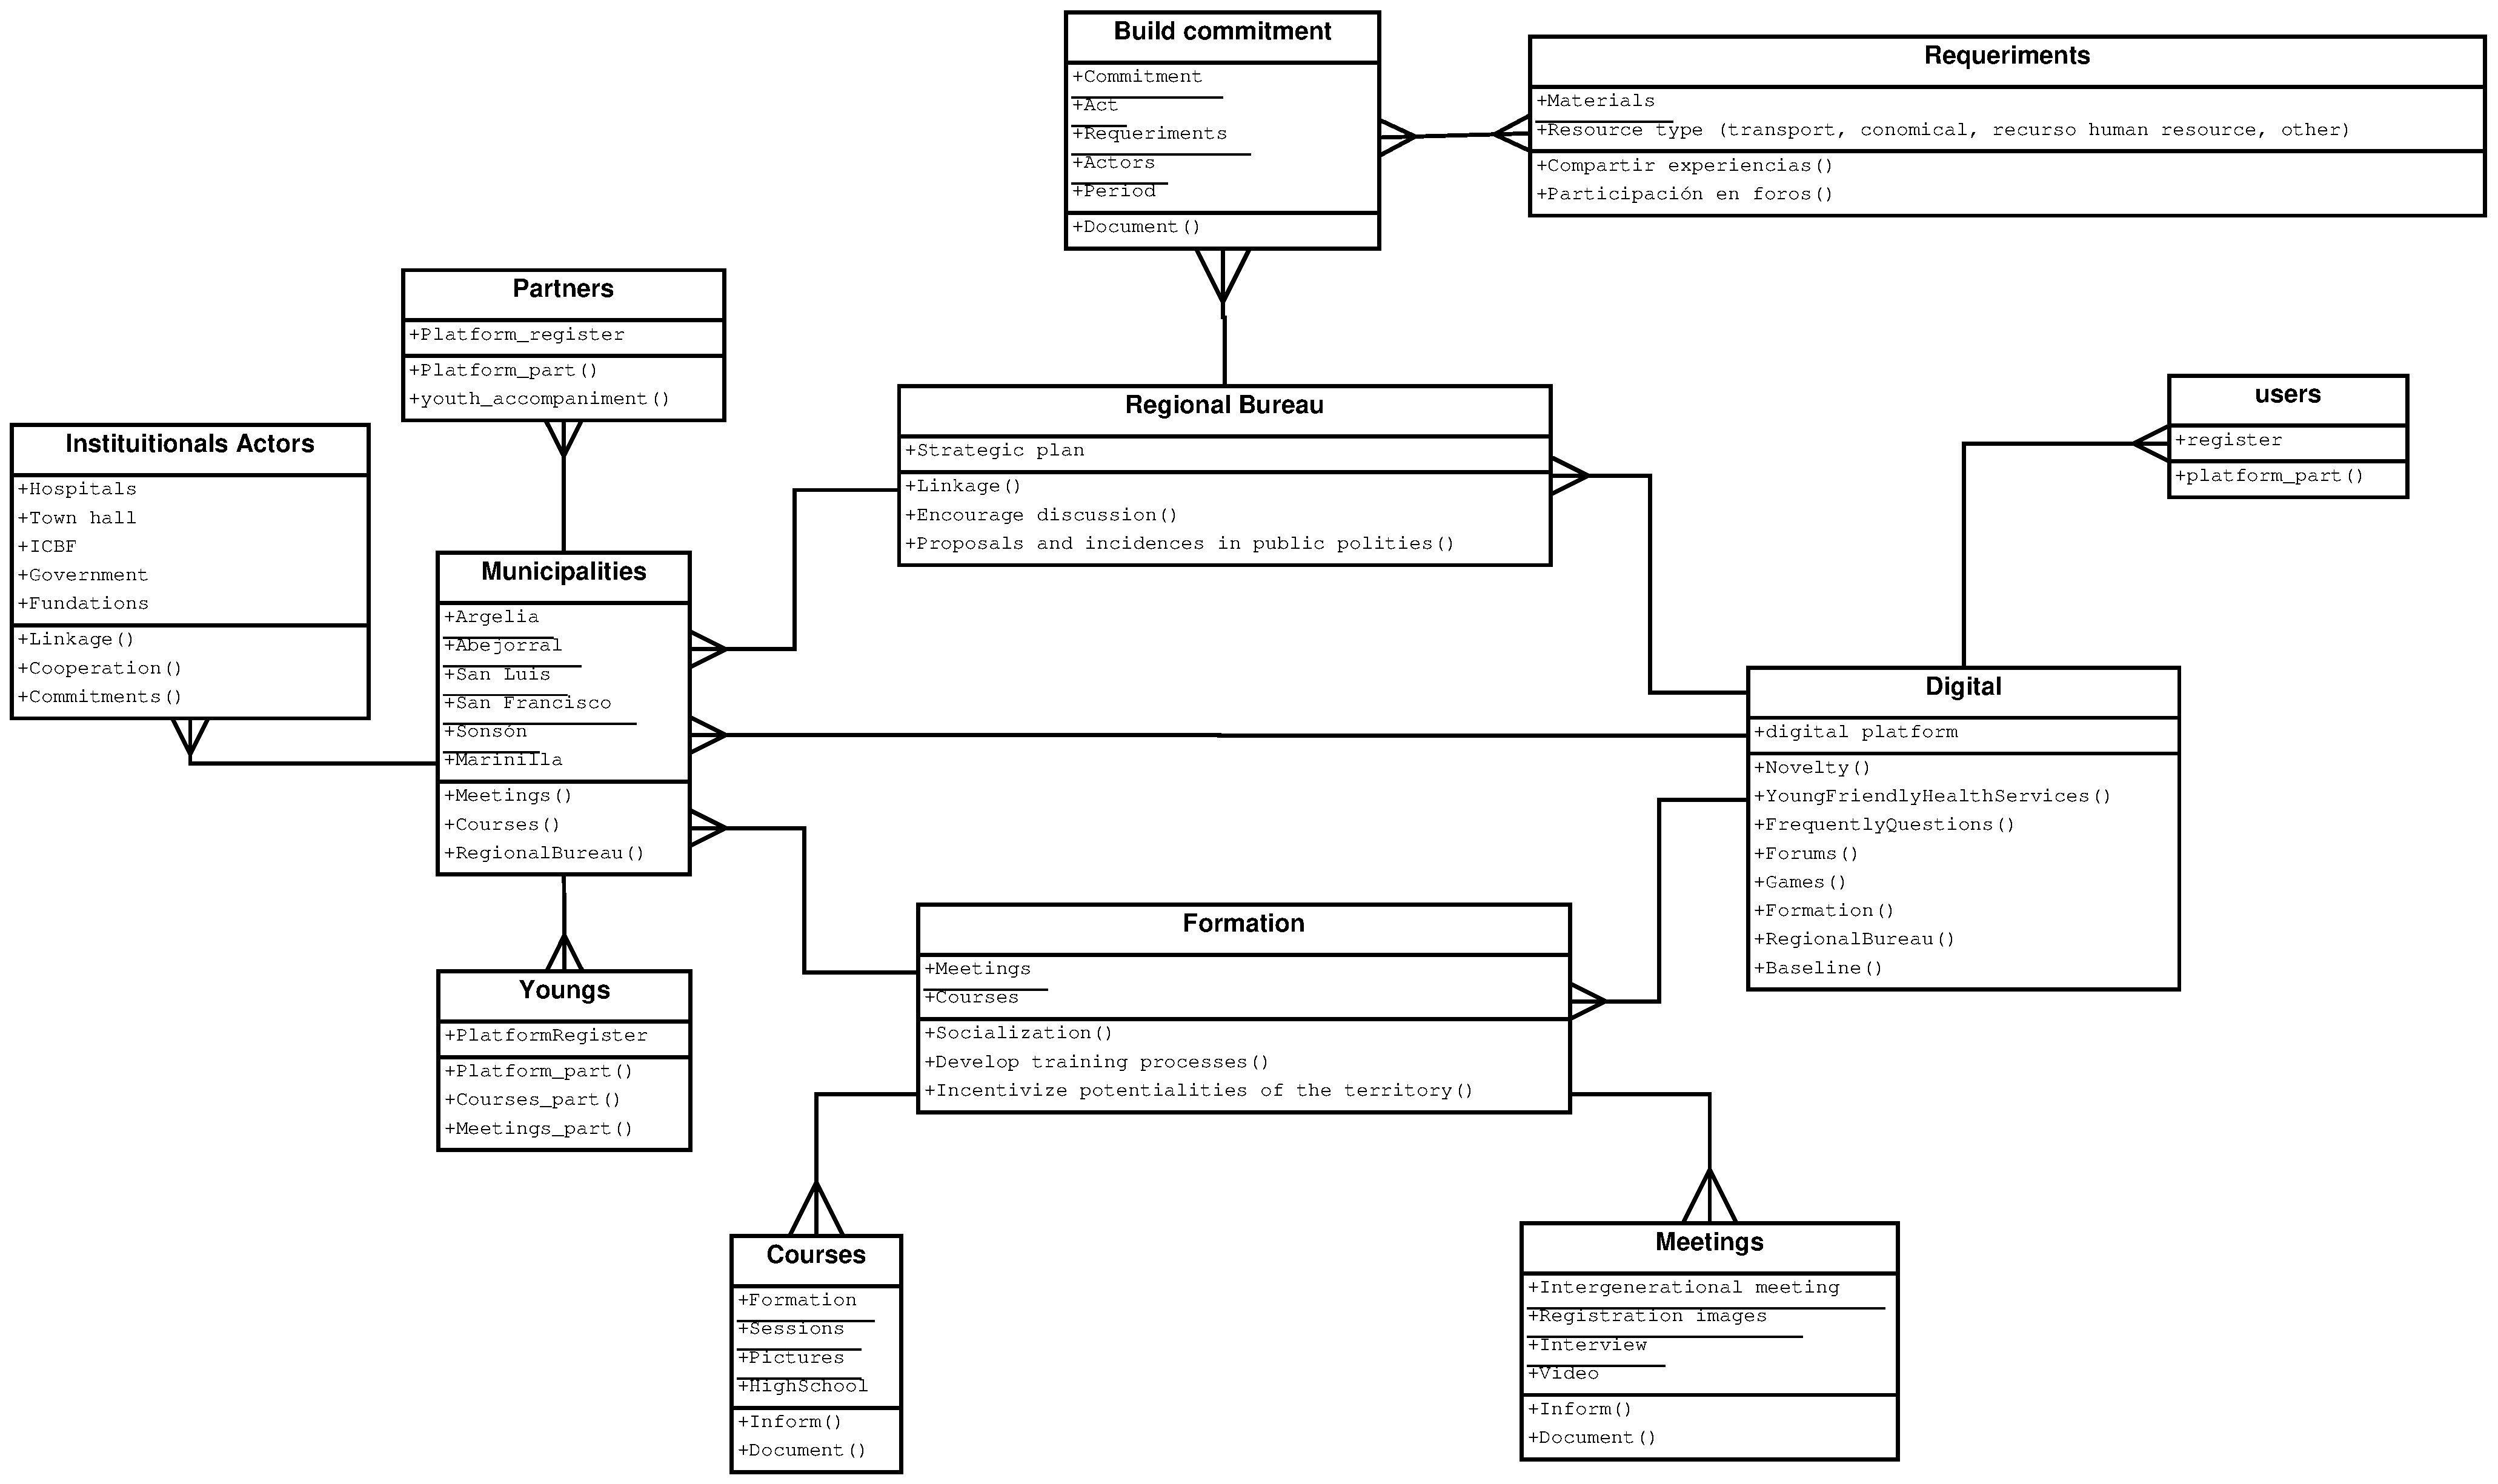
\includegraphics[width=1\linewidth]{red.eps}
\caption{Diagrama relacional.}
\label{fig:red}
\end{figure*}

La estructura base del proyecto de la plataforma digital de la Red Sentir de acuerdo a la manera en como django organiza y dispone los directorios se muestra a continuación:

\fbox{ \parbox{0.85\linewidth}{
\begin{list}{}{}
\item	redsentir/
	\begin{list}{}{}
\item		manage.py
\item		server.py
\item		redsentir/
		\begin{list}{}{}
\item			\underline{\hspace{2mm}}init\underline{\hspace{2mm}}.py
\item			settings.py
\item			urls.py
\item			wsgi.py
		\end{list}
\item faq/
\item formacion/
\item foro/
\item lineabase/
\item lineatiempo/
\item mesa/
\item seguridad/
\item servicios/
\item static/
\item template/
	\begin{list}{}{}
	\item sitio/
	\item base.html
	\end{list}
	\end{list}
\end{list}
}}\vspace{4mm}

Cada una de las carpetas en las que esta dividido el proyecto corresponden a aplicaciones, las cuales contienen los siguientes archivos:

\vspace{4mm}
\fbox{ \parbox{0.85\linewidth}{
\begin{list}{}{}
\item		faq/
		\begin{list}{}{}
\item		\underline{\hspace{2mm}}init\underline{\hspace{2mm}}.py
\item		admin.py
\item		apps.py
\item		migrations/
			\begin{list}{}{}
\item			\underline{\hspace{2mm}}init\underline{\hspace{2mm}}.py
			\end{list}
\item		models.py
\item		test.py
\item		urls.py
\item		views.py
		\end{list}
\end{list}
}}\vspace{4mm}

Dentro de los resultados obtenidos en el desarrollo del proyecto, y que se pueden visualizar en la plataforma digital se encuentran: $(i)$ una plataforma realizada a la medida en funcionamiento, $(ii)$ dos videojuegos en la plataforma, $(iii)$ materiales pedagógicos con acceso virtual, $(iv)$ $30$ foros virtuales para la participación de los adolescentes, $(iv)$ información del proyecto en la plataforma, $(v)$ manifestación de los compromisos de las alcaldías municipales, $(vi)$ vinculación de las instituciones prestadoras de servicios de los municipios, y $(vii)$ constante acompañamiento y solución de inquietudes a los jóvenes a través de la plataforma digital.

La plataforma digital de la Red Sentir logró vincular en sus primeros seis meses de funcionamiento un total de 2511 usuarios (figura~\ref{fig:porcentaje}).

Para observar la aplicación web desarrollada por el componente digital de la Red Sentir, es necesario ingresar en el navegador~\url{www.redsentir.org}, allí se puede observar los diferentes resultados expuestos en el presente artículo.

\begin{figure*}[tbp]
  \centering
	  \subfloat[]{\includegraphics[width=0.48\textwidth]{menor.png}\label{fig:menores}}
	  \hspace{1mm}
 	  \subfloat[]{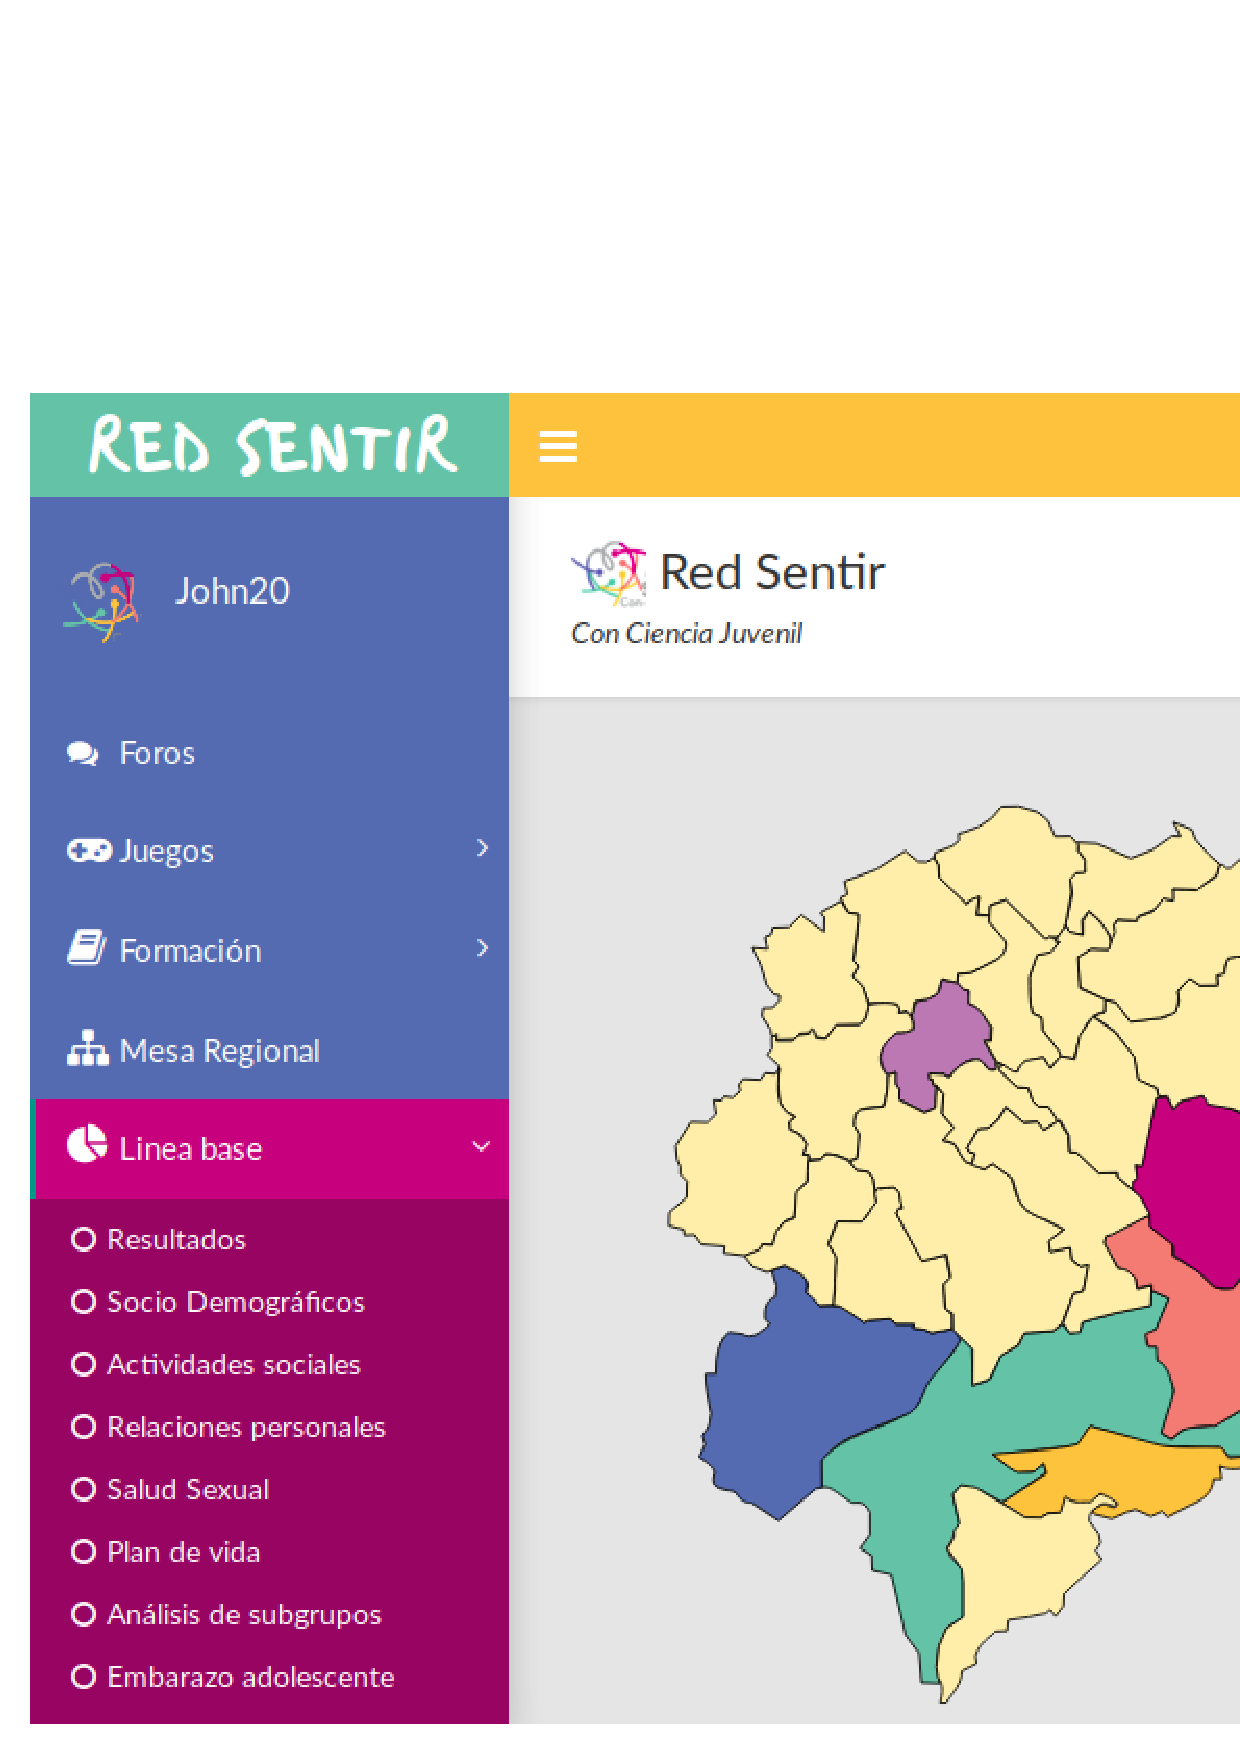
\includegraphics[width=0.48\textwidth]{mayor.png}\label{fig:mayores}}
  \caption{Vista de la plataforma digital según la edad del usuario. (a) Menor de 19 años, (b) mayor de 19 años.}
  \label{fig:vista_plataforma}
\end{figure*}

\begin{figure}[tbp]
\centering
\includegraphics[width=0.48\textwidth]{admin.png}
\caption{Módulo de administración de la Red Sentir.}
\label{fig:admin}
\end{figure}

\begin{figure}[tbp]
\centering
\includegraphics[width=0.48\textwidth]{novedades.png}
\caption{Linea de tiempo de la plataforma Red Sentir.}
\label{fig:novedades}
\end{figure}

\begin{figure}[tbp]
\centering
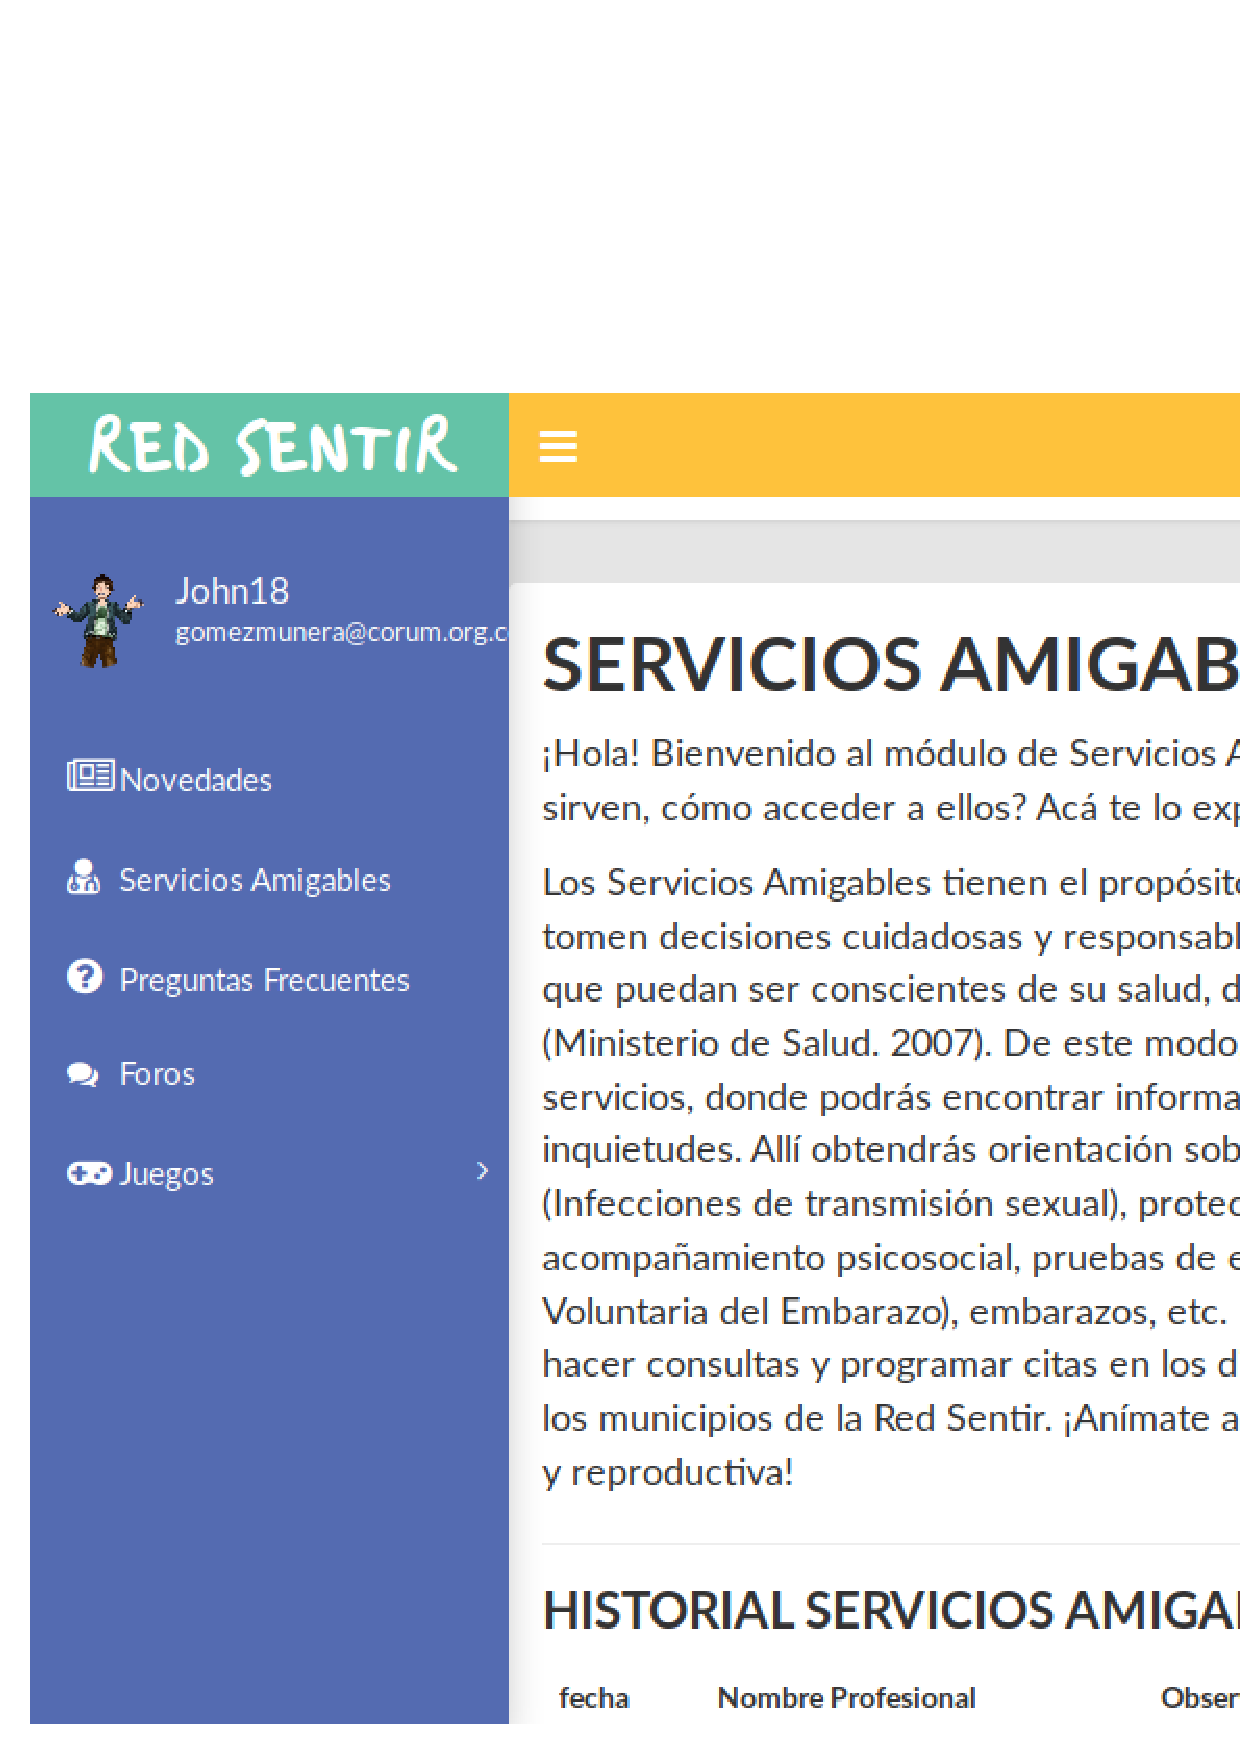
\includegraphics[width=0.48\textwidth]{SA.png}
\caption{Módulo de Servicios Amigables.}
\label{fig:SA}
\end{figure}

\begin{figure}[tbp]
\centering
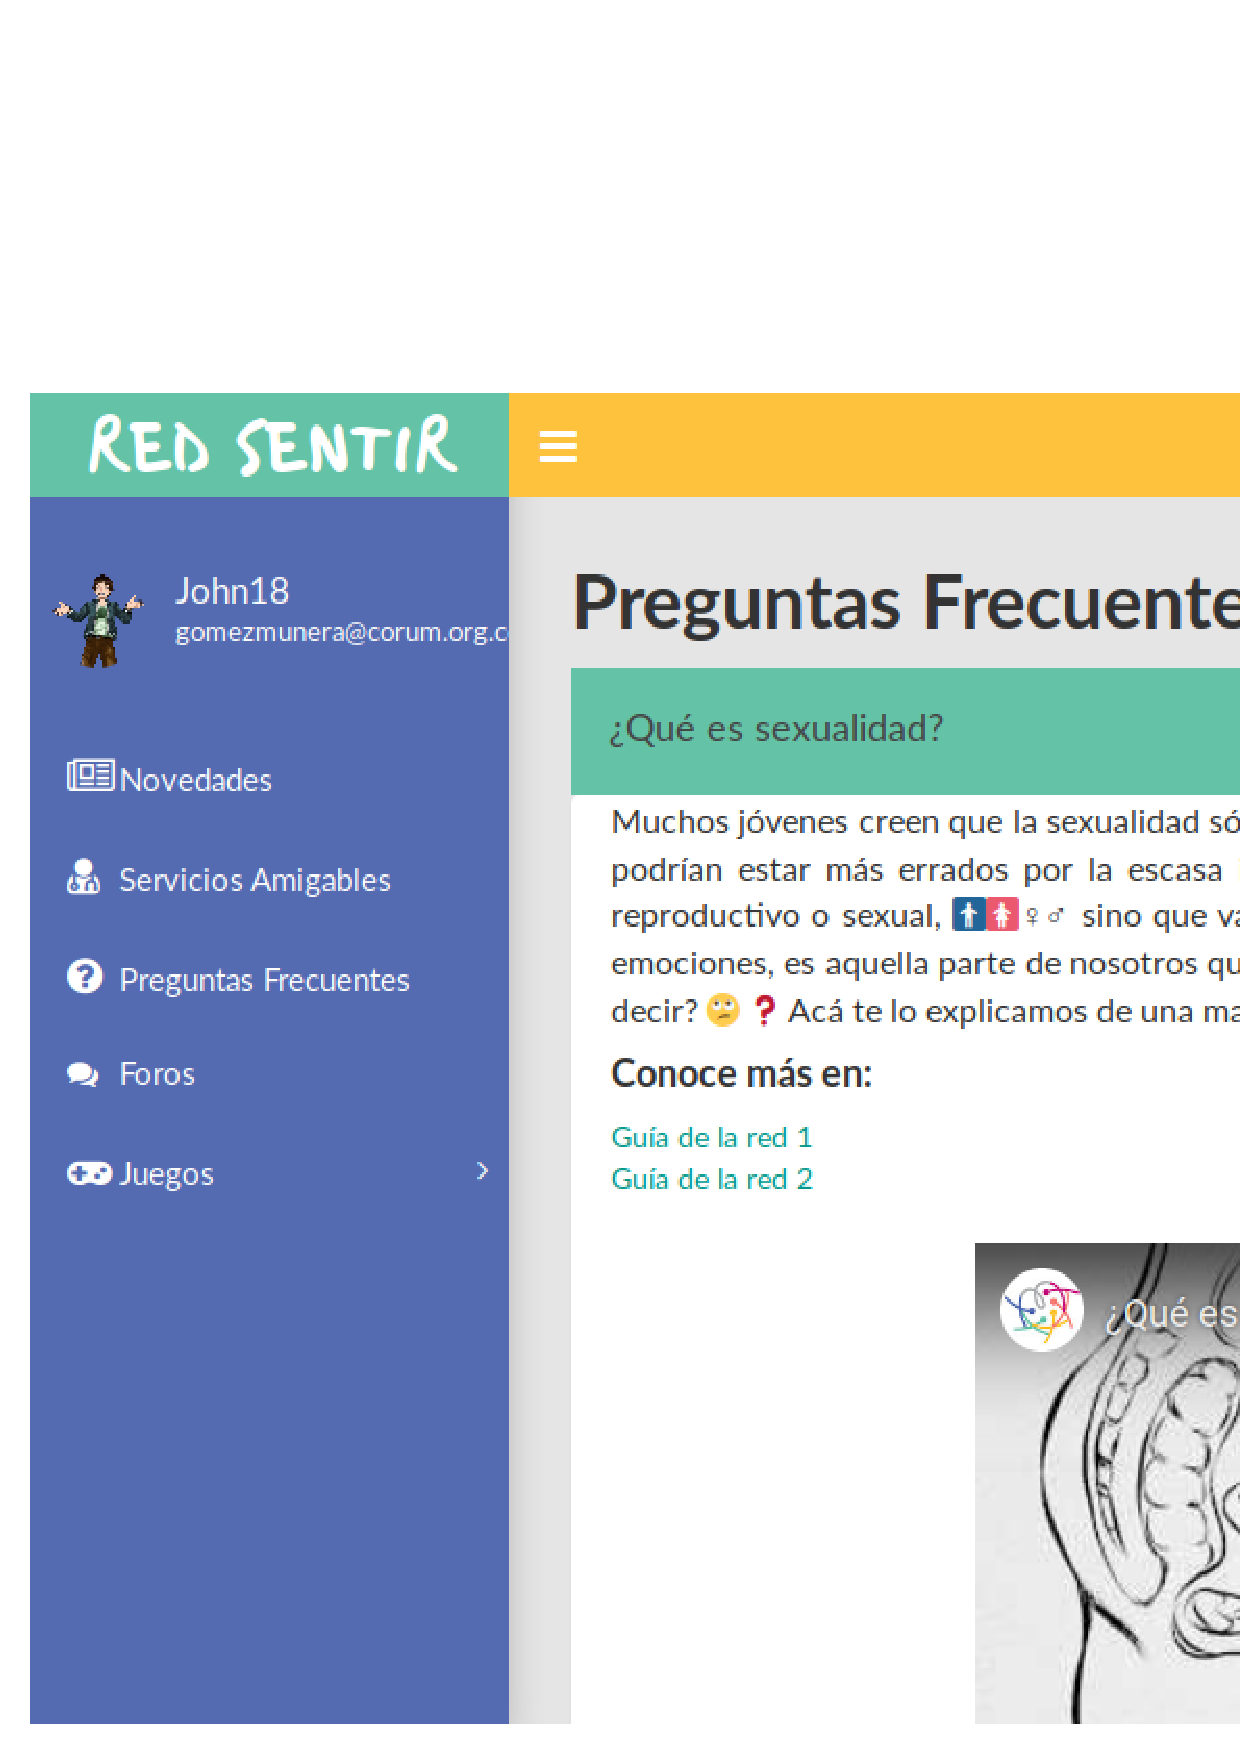
\includegraphics[width=0.48\textwidth]{FAQ.png}
\caption{Módulo de Preguntas Frecuentes.}
\label{fig:FAQ}
\end{figure}

\begin{figure}[tbp]
\centering
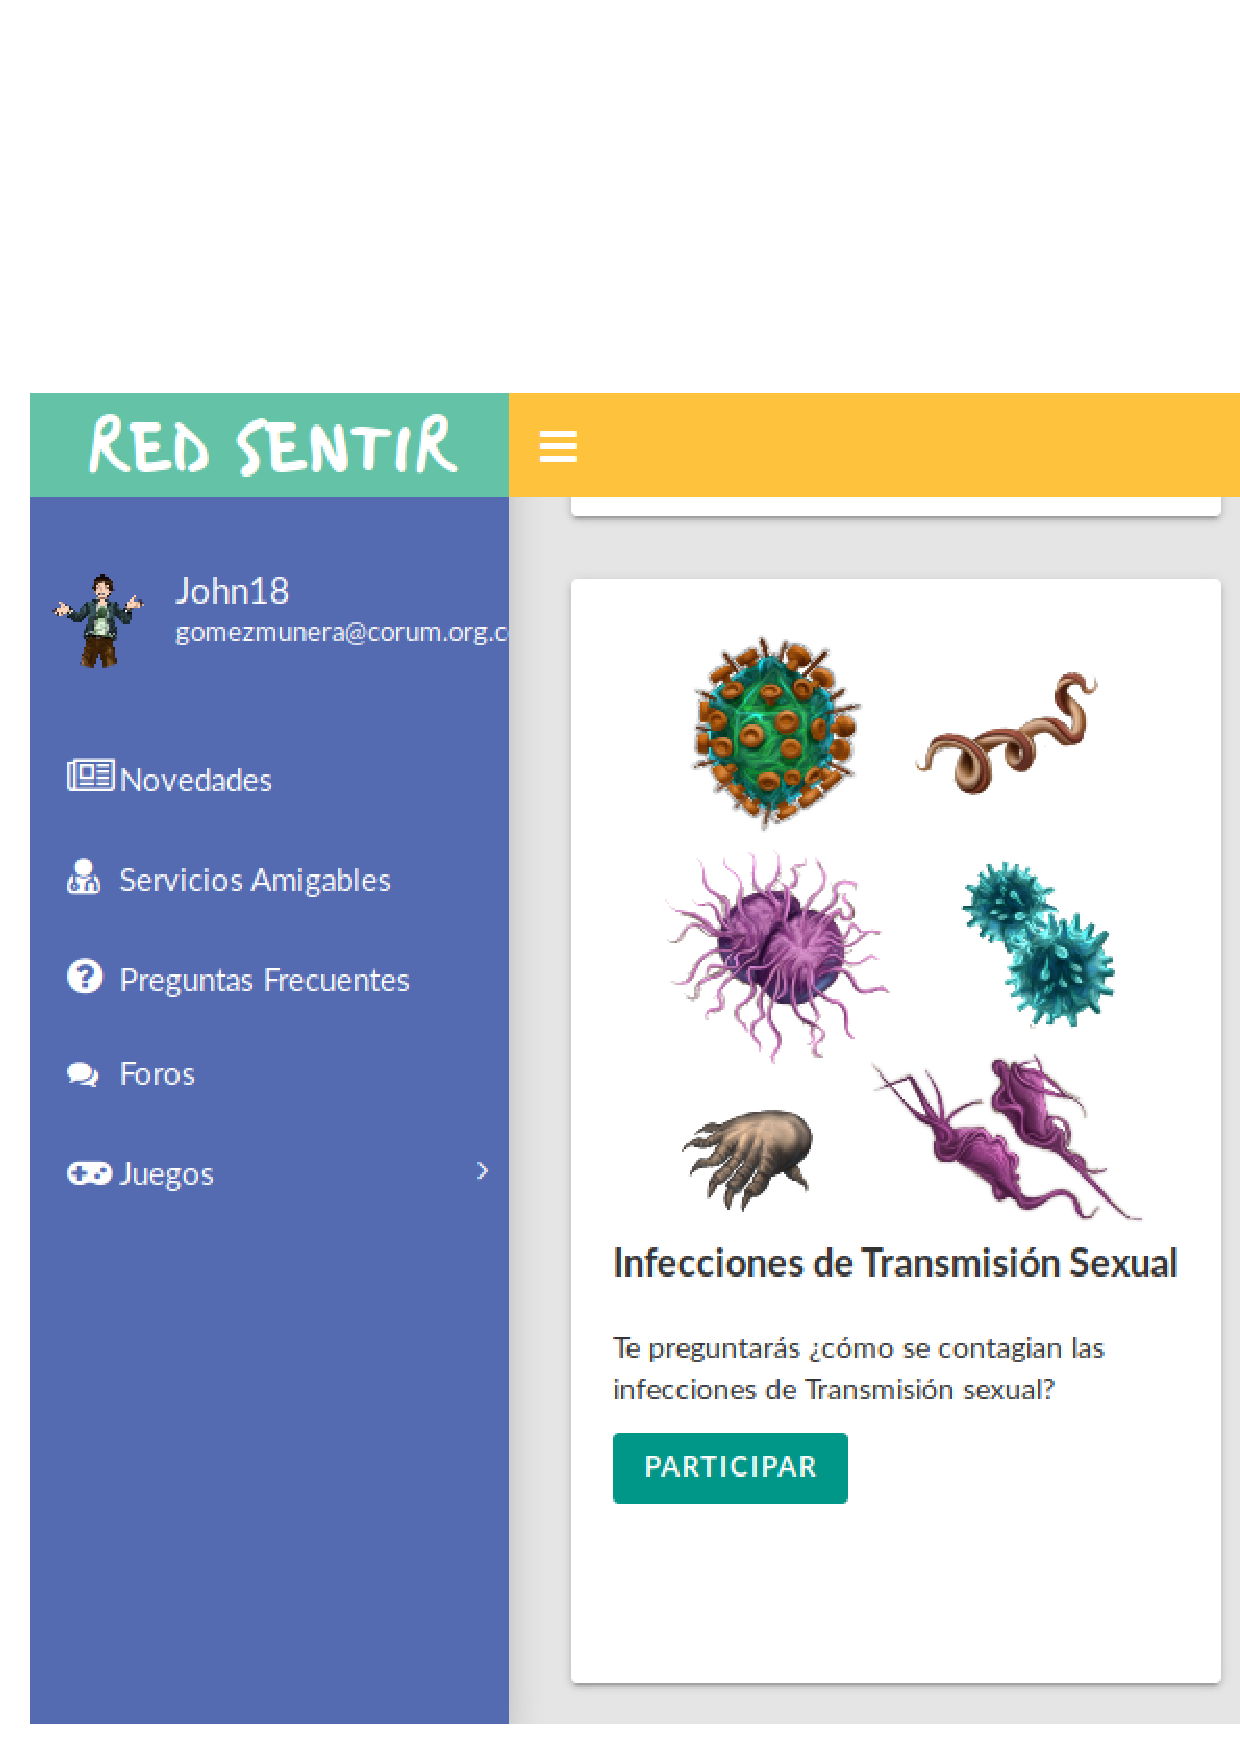
\includegraphics[width=0.48\textwidth]{foros.png}
\caption{Módulo de foros de la Red Sentir.}
\label{fig:foros}
\end{figure}

\begin{figure*}[tbp]
  \centering
	  \subfloat[]{\includegraphics[width=0.48\textwidth]{juego1.png}\label{fig:preventor}}
	  \hspace{1mm}
 	  \subfloat[]{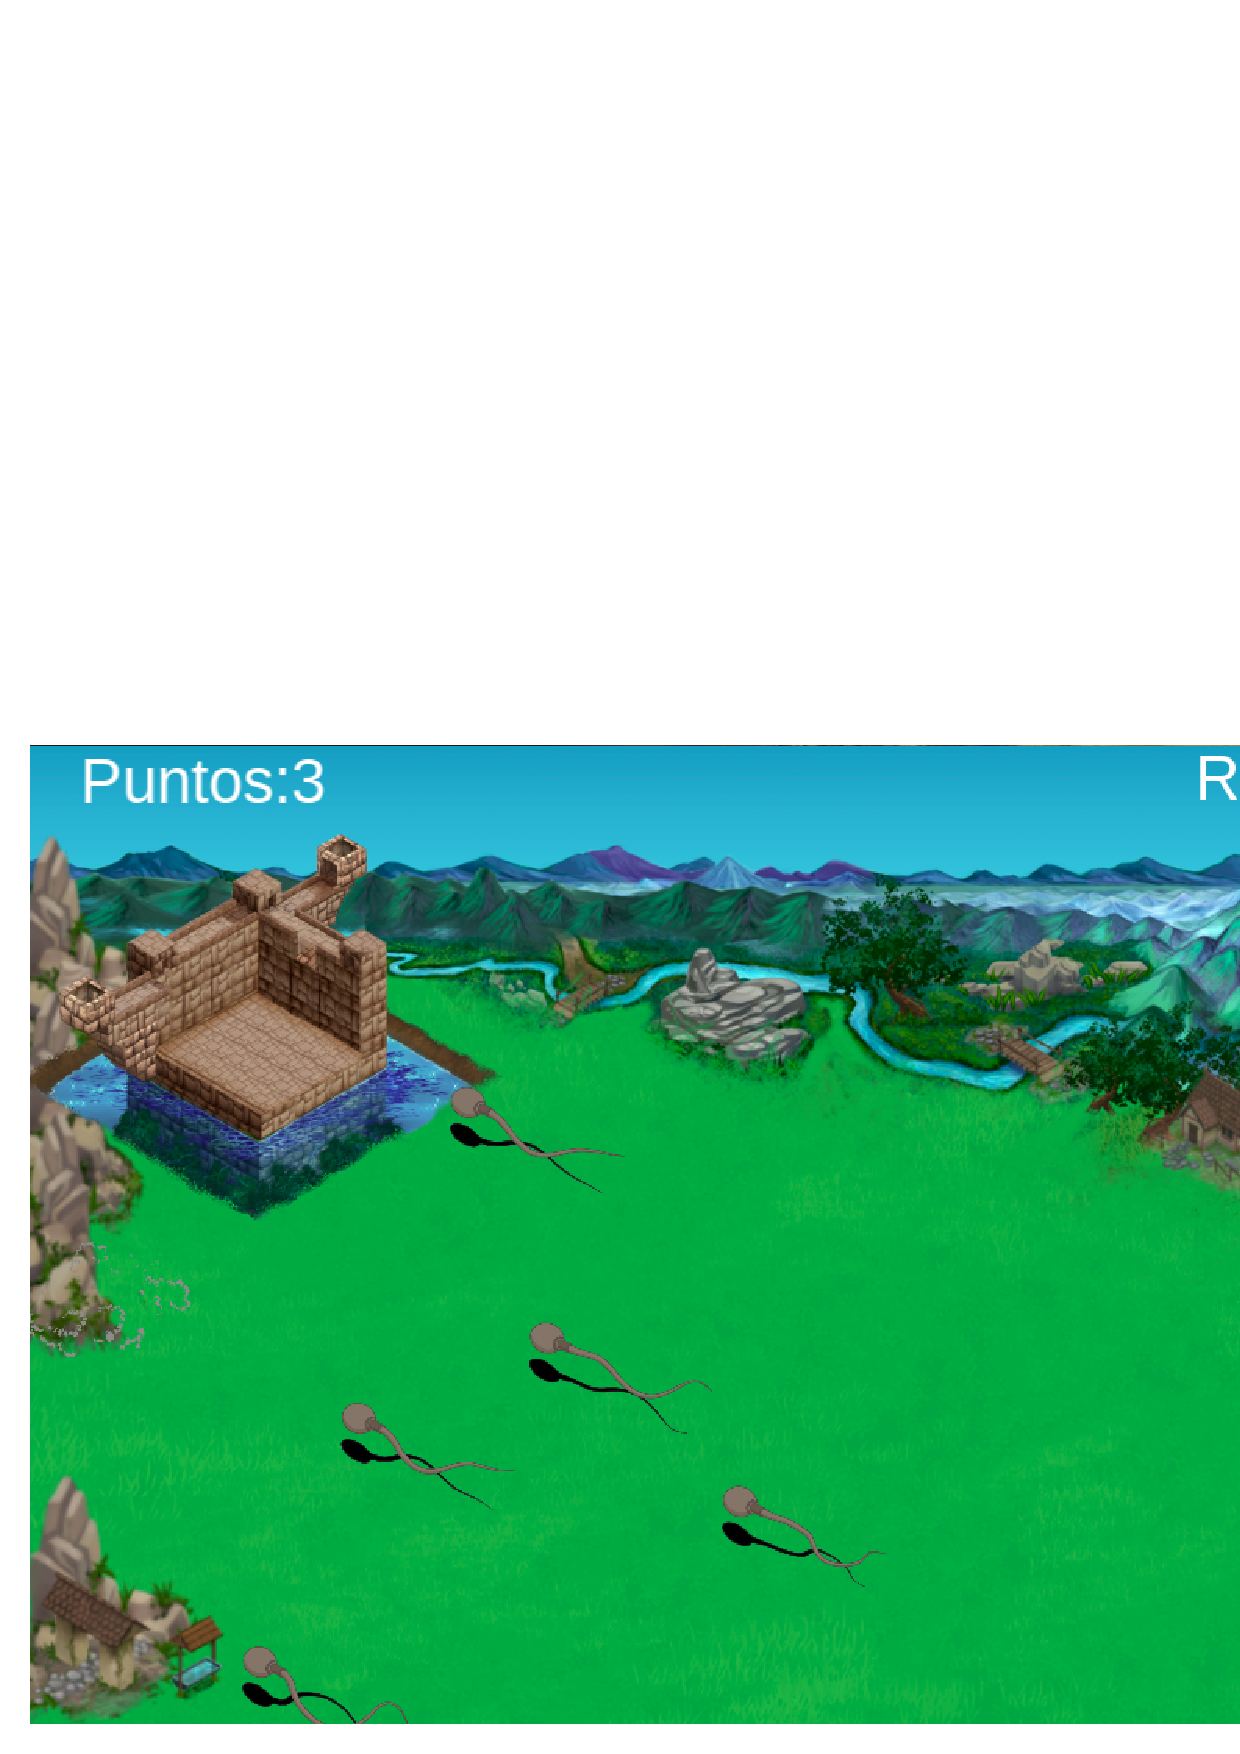
\includegraphics[width=0.48\textwidth]{juego2.png}\label{fig:dawn}}
  \caption{Juegos disponibles en la plataforma digital de la Red Sentir.}
  \label{fig:juegos}
\end{figure*}

\begin{figure*}[tbp]
  \centering
	  \subfloat[]{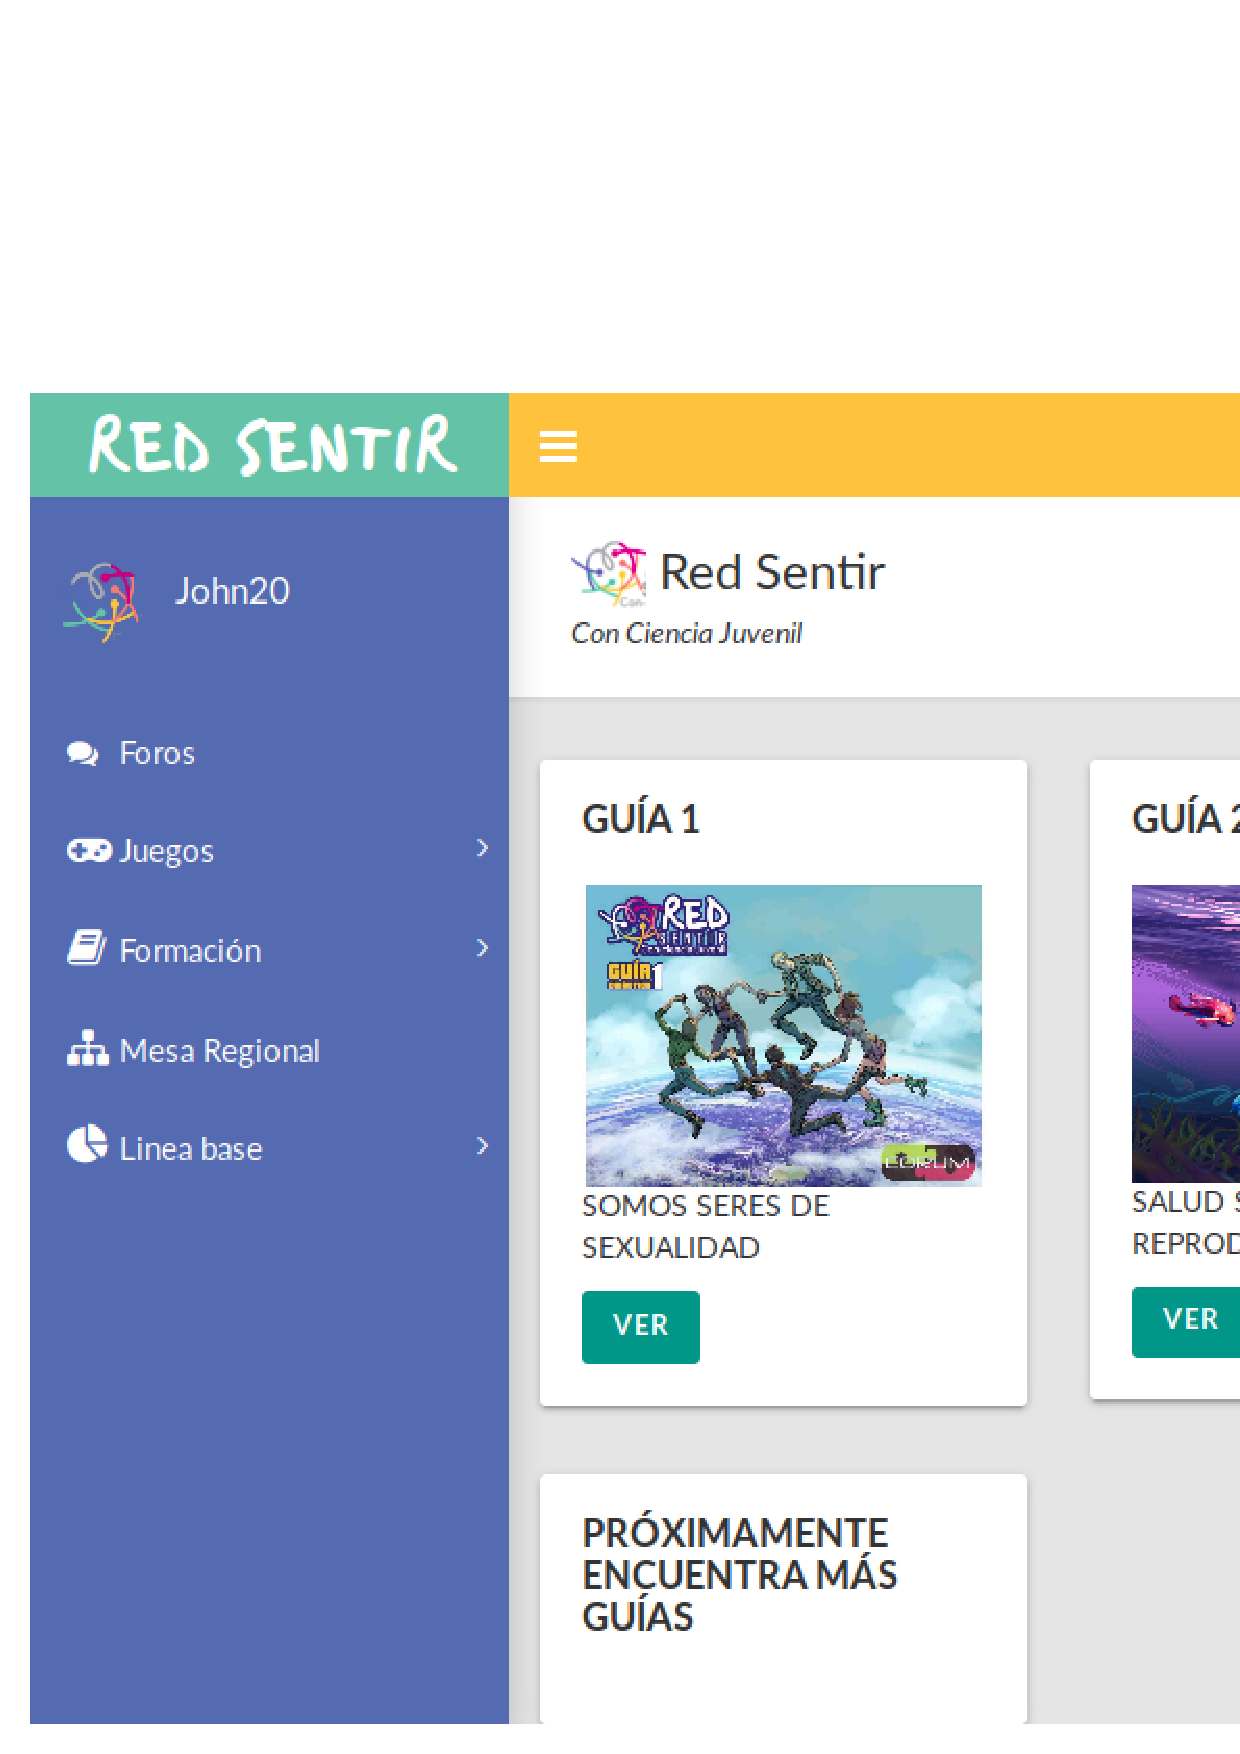
\includegraphics[width=0.48\textwidth]{guias.png}\label{fig:guias}}
	  \hspace{1mm}
 	  \subfloat[]{\includegraphics[width=0.48\textwidth]{encuentros.png}\label{fig:encuentros}}
  \caption{Módulo de formación disponible en la plataforma. (a) Guías de docentes, (b) encuentros locales.}
  \label{fig:formacion}
\end{figure*}

\begin{figure*}[tbp]
  \centering
	  \subfloat[]{\includegraphics[width=0.48\textwidth]{planes.png}}
	  \hspace{1mm}
 	  \subfloat[]{\includegraphics[width=0.48\textwidth]{planes1.png}}
  \caption{Módulo Mesa Regional disponible en la plataforma. }
  \label{fig:mesa}
\end{figure*}

\begin{figure}[tbp]
\centering
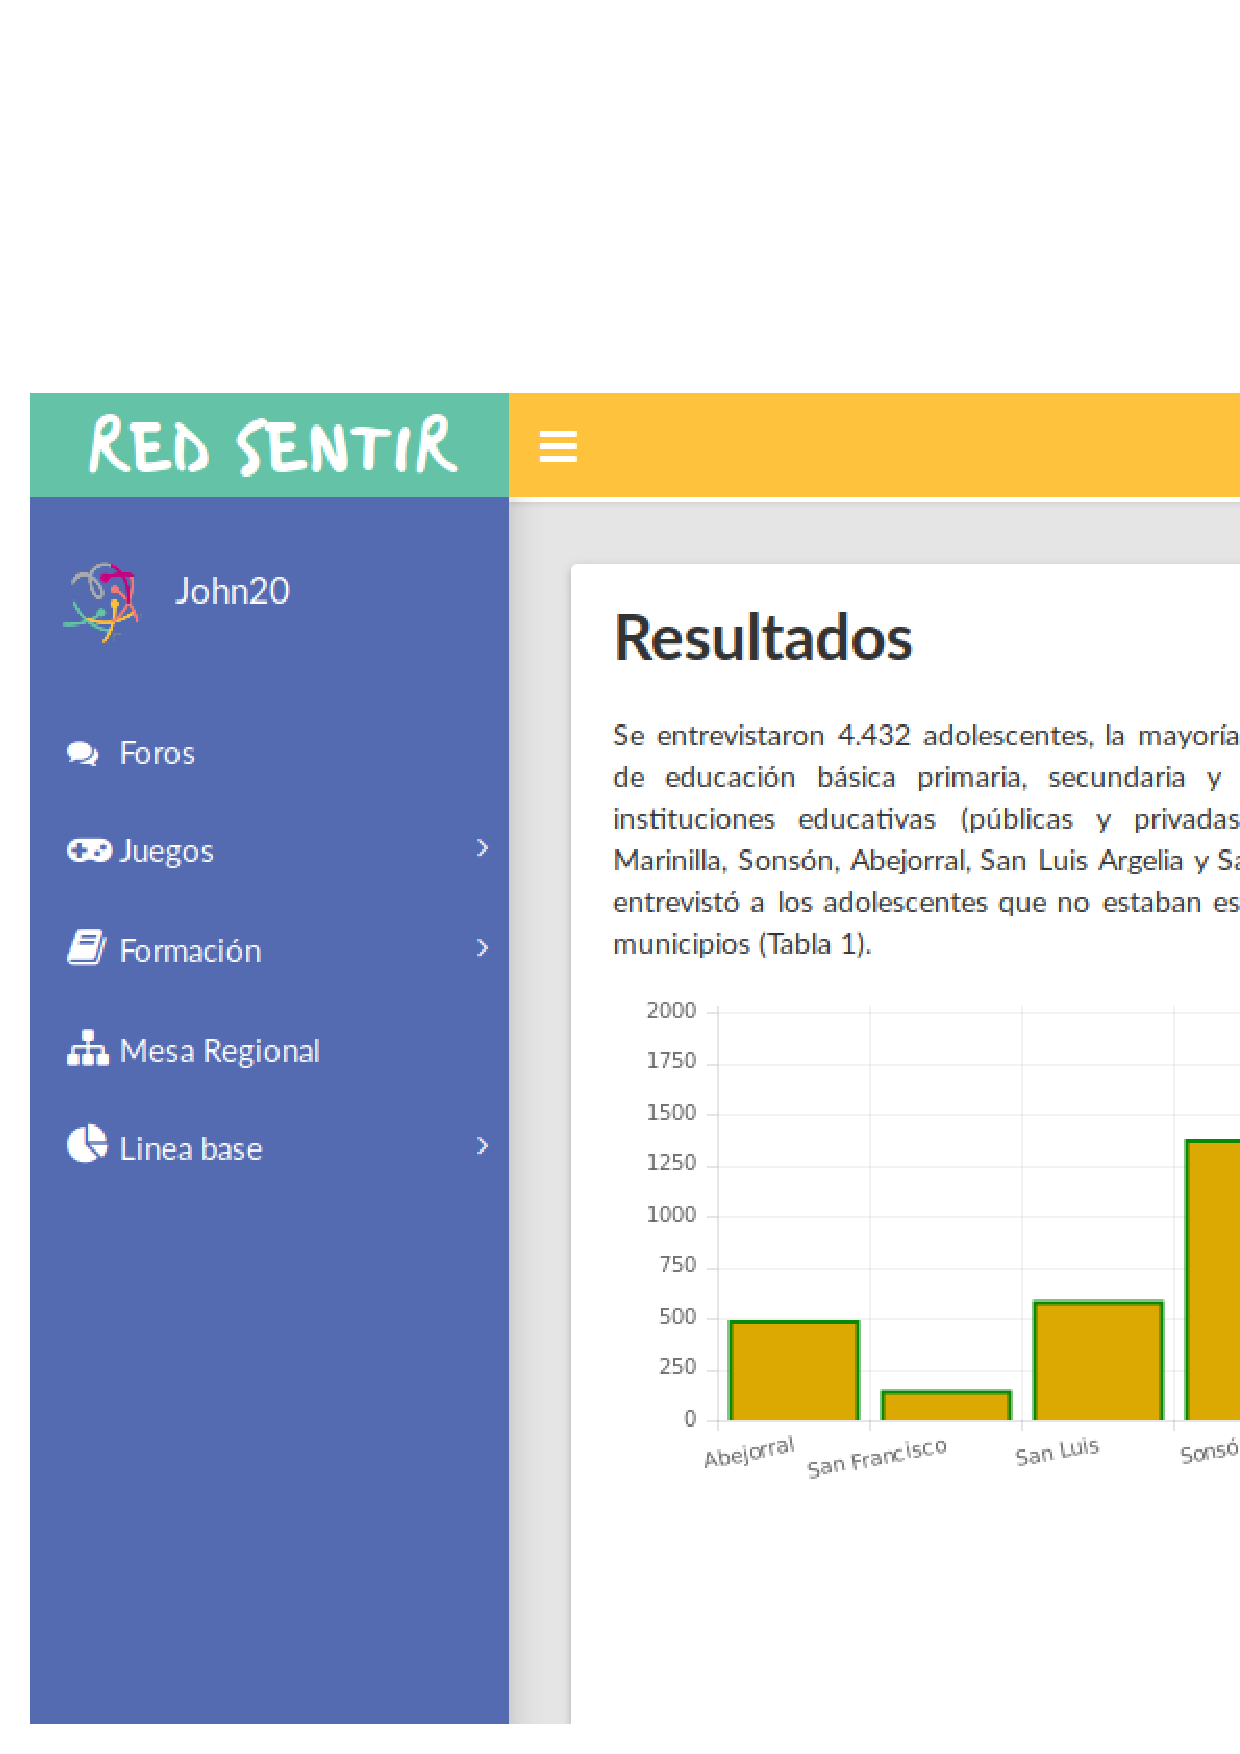
\includegraphics[width=0.48\textwidth]{resultados.png}
\caption{Módulo de Linea base del proyecto.}
\label{fig:lineabase}
\end{figure}

\section{CONCLUSIONES Y PERSPECTIVAS}\label{sec:conclusiones}
La Red Sentir se ha constituido en una estrategia novedosa para el abordaje del fenómeno del embarazo adolescente, fenómeno resultante de diversas problemáticas y caracterizado como un fenómeno de alta complejidad(UNESCO). Responder a esta complejidad requiere de la articulación de acciones de diferentes instituciones de tal forma que se puedan crear impactos sociales favorables, es así como la plataforma digital de la red sentir respondió a estas necesidades y creó herramientas digitales para facilitar las interacciones complejas entre gobiernos, colegios, jovenes, profesores, instituciones de salud y el equipo de la Red Sentir.

La Red Sentir se encuentra alineada con la búsqueda de los gobiernos nacionales por generar una mayor inclusión comunitaria y reducir los factores de riesgos en los que están inmersos muchas de las personas (Sobre todo los más jóvenes), que terminan en muchos de los casos reflejado con consecuencias que pueden truncar el plan de vida de los jóvenes perpetuando los ciclos de pobreza en las comunidades. 

De igual manera, no es solo la situación económica la que influye en los procesos educativos de los adolescentes, sino también  los factores demográficos, sociales, culturales y uno de los más importantes el acceso a las TIC.

Con la investigación realizada por la Red Sentir acerca de los factores de riesgo asociados al fenómeno del embarazo adolescente se generó una estrategia de intervención haciendo énfasis en los planes de vida, los derechos humanos, el reconocimiento del territorio, el cuidado del cuerpo, el aprendizaje y el uso de métodos anticonceptivos y el fortalecimiento de los sueños.

La plataforma virtual complementó el proceso llevado a cabo por el componente de formación como una estrategia para vincular, reforzar y lograr un mayor alcance diferente al logrado con los adolescentes que participaron directamente de los semilleros. 

Desde lo técnico, el uso de los diferentes frameworks, permitieron la programación de una plataforma virtual cuyo objetivo es el de crear confianza en los más jóvenes, al funcionar como una red social orientada directamente a trabajar, hablar y formar sobre los temas de sexualidad, para que los jóvenes obtengan información que les ayude a experimentar, descubrir y vivir la sexualidad de una manera responsable. Con el desarrollo de la plataforma digital, se pudo incorporar y mezclar tecnologías junto 
con los respectivos lenguajes utilizados (Django, cherrypy, HTML, CSS, JavaScript, Postgresql) que llevaron consecuentemente y en buen termino a un resultado final reflejando las fortalezas y carácter interdisciplinar del equipo de la Red Sentir.

Tanto los productos como los resultados obtenidos por el proyecto, arrojan un análisis positivo y satisfactorio en todos los aspectos y desde los diferentes componentes. Esto indica en si, el asentamiento de una base para continuar interviniendo en las comunidades en las que este factor de riesgo es alto, dejando en si un trabajo que puede ser extendido, complementado y replicado para las demás comunidades en los que se considere pertinente implementar la estrategia. Dentro de las funcionalidades que puede tener la plataforma digital, las mismas pueden ampliarse e incorporar nuevas herramientas, ya que esta es una tarea de crecimiento continuo que debe adaptarse a nuevas tecnologías, siendo un proceso iterativo e incremental, aunque precisamente es eso lo que puede verse como una oportunidad, ya que dentro de lo digital, la necesidad de introducir nuevas mejoras y nuevos contenidos que complementen lo ya implementado es lo que permiten que se genere una confianza y un retorno a la plataforma, entre las funcionalidades identificadas para seguir trabajando dentro de la plataforma se plantean:

\begin{itemize}
\item Crear continuamente contenido para los jóvenes, padres y actores institucionales.
\item Volverla una herramienta masiva, que sea implementada en las instituciones educativas dentro de un ámbito nacional, sirviendo de apoyo en la enseñanza de la sexualidad.
\item Vincular a los educadores para generar trabajo colaborativo a través de la plataforma.
\item Mejorar y actualizar los video juegos existentes dentro de la plataforma, incorporando para ello más personas preocupadas por un aprendizaje con diversión, esto tiene que ver con las nuevas estrategias de e-learning, desde las cuales se ha demostrado que cuanto más entretenido se encuentre el estudiante más información puede retener, lo que conlleva que el estudiante puede aprender más y a su vez generarles una apropiación de las TIC de manera eficiente dentro de los entornos educativos.
\item Aumentar la dificultad de los juegos a medida que se va avanzando y consiguiendo puntos. Dicha dificultad puede verse reflejada en mayor velocidad, aparición de nuevos personajes, uso de diferentes herramientas, movimientos, inclusión de nuevas animaciones, inclusión de información educativa o nuevos gráficos.
\item Disponer de una estrategia comercial para compra de elementos que ayuden al autocuidado y a la prevención del embarazo (Anticonceptivos), con el objetivo de ser ofertados a traves de la plataforma y generar sostenibilidad financiera para la misma.
\item Tener un registro de los puntajes obtenidos en los juegos dentro de la base de datos, lo que permitirá tener una mejor estadística de los usuarios y nivel de juego, para realizar tratamientos posteriores.
\end{itemize}

\bibliographystyle{IEEEtran}
\bibliography{biblio_digital}
\end{document}
